\documentclass[a4paper, 11pt]{article}
\usepackage{comment} % enables the use of multi-line comments (\ifx \fi) 
\usepackage{lipsum} %This package just generates Lorem Ipsum filler text. 
\usepackage{fullpage}% changes the margin
\usepackage{amsmath}
\usepackage{kbordermatrix}
\usepackage{hanging}
\usepackage{graphicx}
\usepackage{hyperref}
\usepackage{array}
\usepackage{pdflscape}
\usepackage{rotating}
\usepackage{tabularx}
\usepackage{ragged2e}
\usepackage{longtable}
\usepackage[section]{placeins}




\graphicspath{ {images/} }
\begin{document}
%Header-Make sure you update this information!!!!
\noindent
\large\textbf{Prediciendo Ingresos Fiscales en México}\\
\normalsize Secretaría de Hacienda y Crédito Público \hfill Camilo Arias Martelo\\
Unidad de Política de Ingresos Tributarios\hfill Fecha: 08/16/2019 \\
Supervisión: Dra Gabriela Calderón Guémez \\\\

Durante el Verano de 2019 se llevó a cabo un proyecto de predicción de los ingresos tributarios en la Unidad de Política de Ingresos Tributarios (UPIT) de la Secretaría de Hacienda y Crédito Público (SHCP). En este documento se presentan los objetivos que se plantearon al inicio, la metodología que se siguió, los resultados y los principales hallazgos y avances que se lograron. Al final se presenta una serie de recomendaciones que a juicio del equipo involucrado, servirían para continuar con los esfuerzos de la UPIT de aprovechar cada vez más las tecnologías de análisis de información que están disponibles hoy.\\

De forma general, se llegó cinco conclusiones principales del ejercicio.
\begin{enumerate}
	\item La primera de ellas, es que la elasticidad de recaudación con respecto al Producto Interno Bruto es mayor a la unidad. Esto es cierto tanto para la recaudación primaria como para la recaudación neta. Este comportamiento refleja un incremento constante en la eficiencia de la recaudación, definida como recaudación tributaria como porcentaje del Producto Interno Bruto.
	\item Sería muy importante repetir este ejercicio con los datos de recaudación bruta. La recaudación tributaria en valores netos es un proceso que se ve afectado fuertemente por acciones políticas que dificultan su predicción. De acuerdo con expertos en la Secretaría de Hacienda, el flujo de devoluciones y compensaciones del Servicio de Administración Tributaria (SAT) responde en gran medida a juego entre dos fuerzas: por un lado, existen presiones políticas para lograr los ingresos estipulados en la Ley de Ingresos de la Federación. Por otro lado, existen presiones de los grandes contribuyentes para obtener devoluciones y compensaciones de forma expedita para financiar sus operaciones. Este juego hace que el comportamiento de los ingresos netos se aleje de la lógica que explicaría el ciclo económico. 
	\item Aunado a lo anterior, los ingresos por los diferentes impuestos difieren en su predictibilidad. De acuerdo con los modelos estimados, la recaudación neta por el ISR es mucho más predecible que la recaudación por IVA, Impuesto a las Importaciones e IEPS. Presumiblemente, esto es resultado de la naturaleza de cada uno de estos impuestos, y de la relevancia que tienen los gastos fiscales en cada uno de ellos.
	\item Los modelos econométricos son, en general, una representación más precisa de la dinámica recaudatoria que los de \textit{Machine Learning} que se usaron. Esta conclusión es positiva, pues ha sido la metodología seguida por la SHCP para pronosticar los ingresos tributarios. No obstante, hay que tomar este ejercicio como un primer esfuerzo y no como un veredicto final. En específico, se recomienda probar enfoques de \textit{Deep Learning} y comparar los resultados. 
	\item Los avances logrados por la UPIT, transitando hacia un mayor uso de las herramientas de análisis de información, hacia la automatización de procesos de análisis, y hacia la consolidación de bases de datos ordenadas, consistentes y confiables son de suma importancia. Otro de los proyectos realizados durante este Verano consolidó el UPIT \textit{Data Lab} v. 1.0 para la consulta de datos de recaudación que será fundamental para el trabajo de análisis de política tributaria. De igual manera, las herramientas de descarga, limpieza, análisis y predicción, y las capacidades de \textit{Python} que se desarrollaron en el equipo analista que resultaron de este proyecto tienen el potencial de incrementar la productividad del equipo de análisis. Para continuar avanzando en esta dirección, el equipo identificó dos áreas estratégicas de inversión:
	\begin{enumerate}
		\item Invertir en la integración de Bases de Datos del SAT con la UPIT. Transitar de un modelo de envío de reportes mensuales por correo electrónico a un modelo en el que el equipo analista pueda consultar la información que la Tesorería de la Federación y el SAT administran en tiempo real. Este proceso de democratización de la información incrementará la productividad del equipo de la UPIT pues disminuirá las barreras que existen en el acceso de la información.
		\item Continuar con la capacitación del equipo en lenguajes de programación como \textit{Python} o \textit{R}. En estos meses de proyecto, donde se dieron capacitaciones semanales de \textit{Python} al equipo, se lograron avances muy importantes. Un analista que no tenía conocimientos de programación realizó su primer análisis de política tributaria en este lenguaje. El equipo analista está formado por los mejores economistas que están egresando actualmente, por lo que seguir invirtiendo en su capacitación en estas herramientas dará resultados cada vez más relevantes y más rápidos en la productividad.
	\end{enumerate}
\end{enumerate}

\section*{Objetivos}
El objetivo general del proyecto fue utilizar los mejores modelos estadísticos para predecir los ingresos tributarios del Gobierno Federal, evaluando diferentes enfoques econométricos y de \textit{Machine Learning} en el desempeño que habrían tenido históricamente. Se incluyeron en el análisis los ingresos tributarios totales, los ingresos tributarios sin el Impuesto Especial sobre Producción y Servicios de hidrocarburos, los ingresos por el Impuesto Sobre la Renta (ISR), por el Impuesto al Valor Agregado (IVA), por el Impuesto a las Importaciones, y por los Impuestos sobre Productos y Servicios sin incluir el relacionado con hidrocarburos (IEPS sin gasolinas). Para lograr el objetivo, se planteó una serie de objetivos específicos que se describen a continuación:
\begin{enumerate}
	\item Estimar con modelos econométricos y de \textit{Machine Learning} los ingresos tributarios de los úitmos meses de cada año y del año siguiente desde 2015 hasta 2018. 
	\item Evaluar la precisión de cada una de esas predicciones, comparándolas con los valores observados.
	\item Seleccionar los mejores modelos para cada uno de los ingresos tributarios.
	\item Estimar el cierre de 2019 para cada uno de los ingresos tributarios usando los modelos con mejor ajuste.
\end{enumerate}
\section*{Los ingresos tributarios}
Para construir un poco de contexto alrededor del proyecto, los ingresos del Gobierno Federal en México ascendieron a 4 billones de pesos del 2019, equivalentes a 17.6\% del Producto Interno Bruto. De estos, los ingresos tributarios representaron 3.17 billones de pesos (13.9\% del PIB) y los ingresos no tributarios 834 miles de millones de pesos (3.7 \% del PIB).  En la figura \ref{fig:ing_gob_fed} podemos ver una serie de los ingresos del gobierno federal como \% del Producto Interno Bruto desde 1990, así como los ingresos tributarios sin el IEPS a las gasolinas, los ingresos no tributarios y el IEPS a las gasolinas. Es interesante analizar el incremento que los ingresos del gobierno federal y los ingresos tributarios han tenido en términos de \% del PIB.

\begin{figure}[hbt!]
    \centering
     \caption{Ingresos del Gobierno Federal}
     \label{fig:ing_gob_fed}
     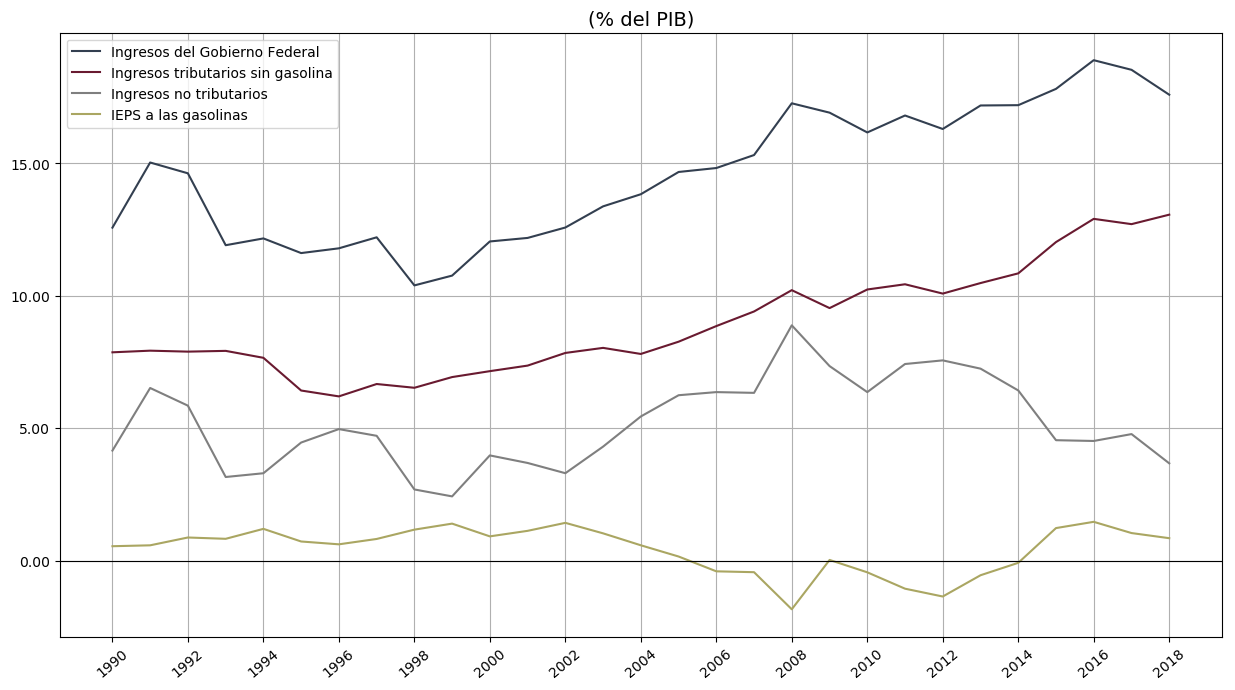
\includegraphics[scale = 0.4]{figures/ingresos_gob_fed}
\end{figure}
Dentro de los ingresos tributarios, el ISR es el que aporta la mayor cantidad, con 1.7 billones de pesos en 2018, seguido por el IVA con 950 miles de millones de pesos. Estos dos impuestos representan 54\% y 30\% de los ingresos tributarios respectivamente. El IEPS a las gasolinas es el tercero en importancia, aportando 193 miles de millones de pesos en 2018, seguido del IEPS al resto de los productos y servicios con 163 miles de millones de pesos. Representan 6\% y 5\% de los ingresos tributarios respectivamente. En la figura \ref{fig:impuestos_perc_trib} se pueden ver estos datos desde 1990. Es interesante resaltar el periodo entre 2005 y 2014, cuando el impuesto a las gasolinas era negativo.

\begin{figure}[hbt!]
    \centering
     \caption{Ingresos tributarios del Gobierno Federal}
     \label{fig:impuestos_perc_trib}
     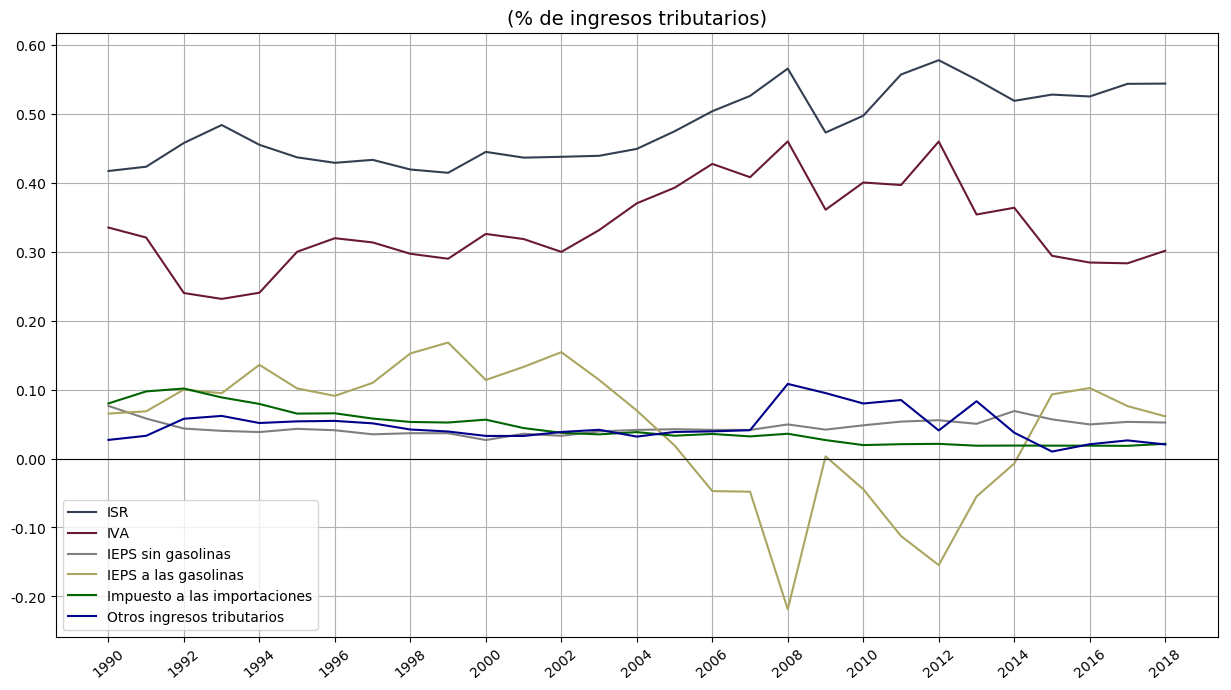
\includegraphics[scale = 0.4]{figures/impuestos_perc_trib}
\end{figure}

Como se mencionó, la elasticidad de los ingresos tributarios con respecto al PIB supera a la unidad. El incremento en el porcentaje que los ingresos tributarios representan del PIB que se ve en la figura \ref{fig:ing_gob_fed} demuestra este punto. Además, para ver más clara la trayectoria que ha seguido el PIB y los ingresos tributarios Gobierno Federal, construimos un índice que elimina la diferencia de magnitudes. De 2005 a 2018 la economía ha crecido 36.5\%, mientras que 
los ingresos tributarios lo han hecho en 125.4\%, resaltando el comportamiento del ISR que se ha elevado en 173\%.  En la figura \ref{fig:indice_pib_impuestos_netos} presentamos estas series.
\begin{figure}[hbt!]
    \centering
     \caption{Índice del PIB y de los ingresos tributarios }
     \label{fig:indice_pib_impuestos_netos}
     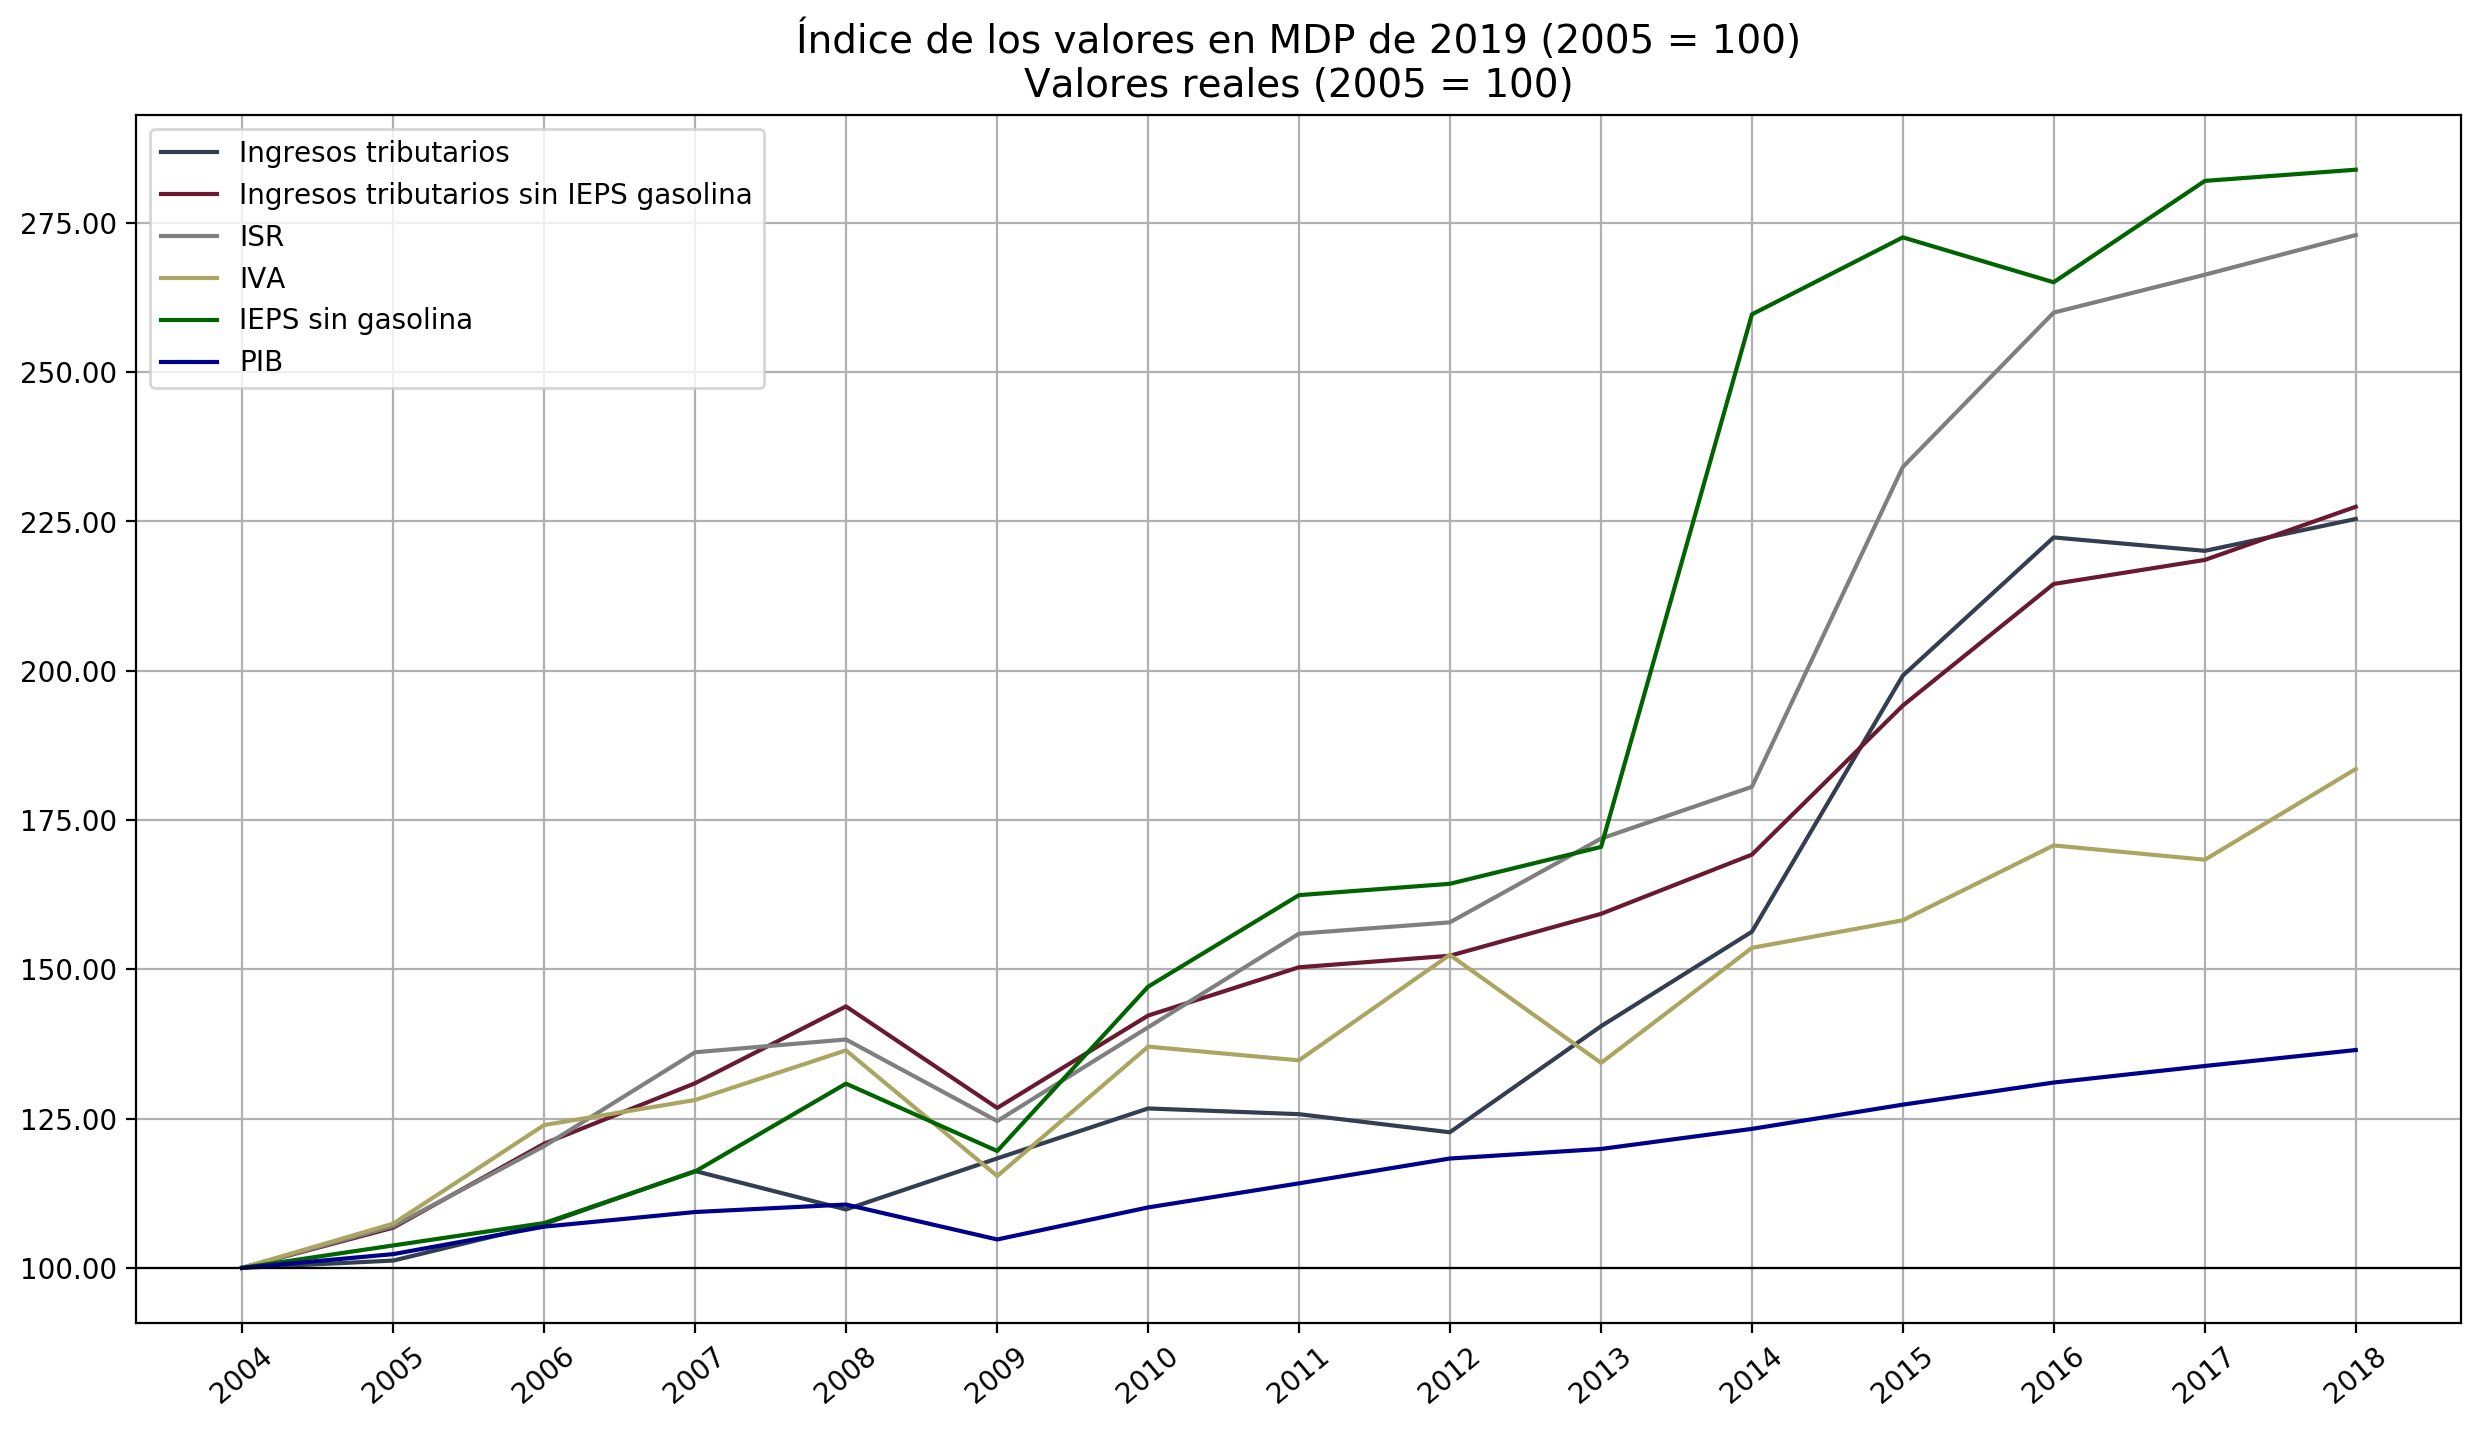
\includegraphics[scale = 0.4]{figures/indice_pib_impuestos_netos}
\end{figure}

La elasticidad recaudación-PIB, desde 2016 a 2018 se presenta en la tabla \ref{tab:elast}. Se excluyén los datos de 2015 para no contaminar las elasticidades con los efectos de la reforma tributaria de 2014. Se puede ver que la elasticidad de los ingresos ha sido mayor a 2 para el ISR, el IVA y los ingresos tributarios sin IEPS gasolina, y de 1.58 para los ingresos tributarios totales.
\begin{table}
\centering
\caption{Elasticidad de ingresos tributarios con respecto al PIB}
 \begin{tabular}{ m{2 cm}  m{1.5cm}  m{1.5cm}  m{1.5cm}  m{1.5cm}  m{1.5cm}  m{1.5cm} } 
 Año & Ingresos trib. & Ingresos trib. sin IEPS gas. & ISR & IVA & IEPS sin gas. & IEPS gas.\\ [0.5ex] 
 \hline \hline
 2016 & 3.99 & 3.6 & 3.8 & 2.7 & -0.95 & 7.8 \\ 
 \hline
 2017 & -0.48 & 0.89 & 1.15 & -0.66 & 3.02 & -12.47\\
 \hline
 2018 & 1.22 & 2.04 & 1.25 & 4.52 & 0.33 & -8.81 \\
 \hline\hline
 Prom. & 1.58 & 2.18 & 2.07 & 2.19 & 0.8 & -4.5 \\
 \hline \hline
\end{tabular}
\label{tab:elast}
\end{table}

\section*{Metodología}
Los primeros dos objetivos específicos se relacionan con identificar los mejores modelos predictivos. Para ello, estimamos y evaluamos un alto número de modelos para cada variable. En esta sección, presentaremos los detalles de este procedimiento. Comenzaremos con las variables en las que nos enfocamos, seguiremos con el proceso general de estimación y evaluación, después explicaremos los modelos que estimamos y finalizaremos con las variables exógenas en las que nos apoyamos.
\subsection*{Variables de interés}
Para la predicción se utilizaron los ingresos tributarios netos con frecuencia mensual desde 1990 disponibles en las \href{http://www.shcp.gob.mx/POLITICAFINANCIERA/FINANZASPUBLICAS/Estadisticas_Oportunas_Finanzas_Publicas/Paginas/unica2.aspx}{Estadísticas Oportunas de las Finanzas Públicas}. Como variables explicativas de los modelos econométricos, se utilizaron del  Banco de Información Económica del \href{https://www.inegi.org.mx/sistemas/bie/}{Instituto Nacional de Estadística e Información}:
\begin{itemize}
\item Indicador Global de la Actividad Económica (IGAE) ajustado por estacionalidad
\item Índice Nacional de Precios al Consumidor, mensual.
\item Valor de las importaciones de bienes y servicios de México.
\item Indicador mensual de consumo
\end{itemize}
Del Sistema de Información Económica del \href{http://www.banxico.org.mx/SieInternet/}{Banco de México}:
\begin{itemize}
\item Tipo de cambio con respecto al dólar promedio mensual.
\item La tasa de interés de los Certificados de Tesorería (CETES) de vencimiento a 91 días promedio mensual.
\end{itemize}
Y del \textit{Federal Reserve Economic Data (FRED)} de la \href{https://fred.stlouisfed.org/}{Reserva Federal de San Luis}:
\begin{itemize}
\item Índice de Precios al Consumidor de Estados Unidos
\item Índice de Producción Industrial de Estados Unidos
\item Índice de Precios de las materias primas global
\item Tasa de interés de los Bonos del Tesoro de Estados Unidos con vencimiento a 3 meses
\item Índice del tipo de cambio del dólar ponderado por nivel de comercio.
\end{itemize}


\subsection*{Criterio de selección}
Cada una de las variables se estimó recaudatorias se estimó con cada uno de los modelos en cuatro momentos anteriores. En la figura se detallan estos cuatro momentos, identificados por cada uno de los renglones. Los cortes fueron junio de 2015, junio de 2016, junio de 2017 y junio de 2018. Cada estimación se hizo simulando que en verdad nos encontrábamos en ese momento y que no conocíamos el futuro. Por ejemplo, para junio de 2015, predecimos la recaudación de los julio a diciembre de 2015 y la recaudación mensual del 2016. Posteriormente, comparamos las predicciones obtenidas con los valores reales de recaudación que es observaron, y construimos medidas de precisión para cada uno de los modelos. 
\begin{figure}[hbt!]
    \centering
     \caption{Procedimiento de selección de modelos}
     \label{fig:cross_validation}
     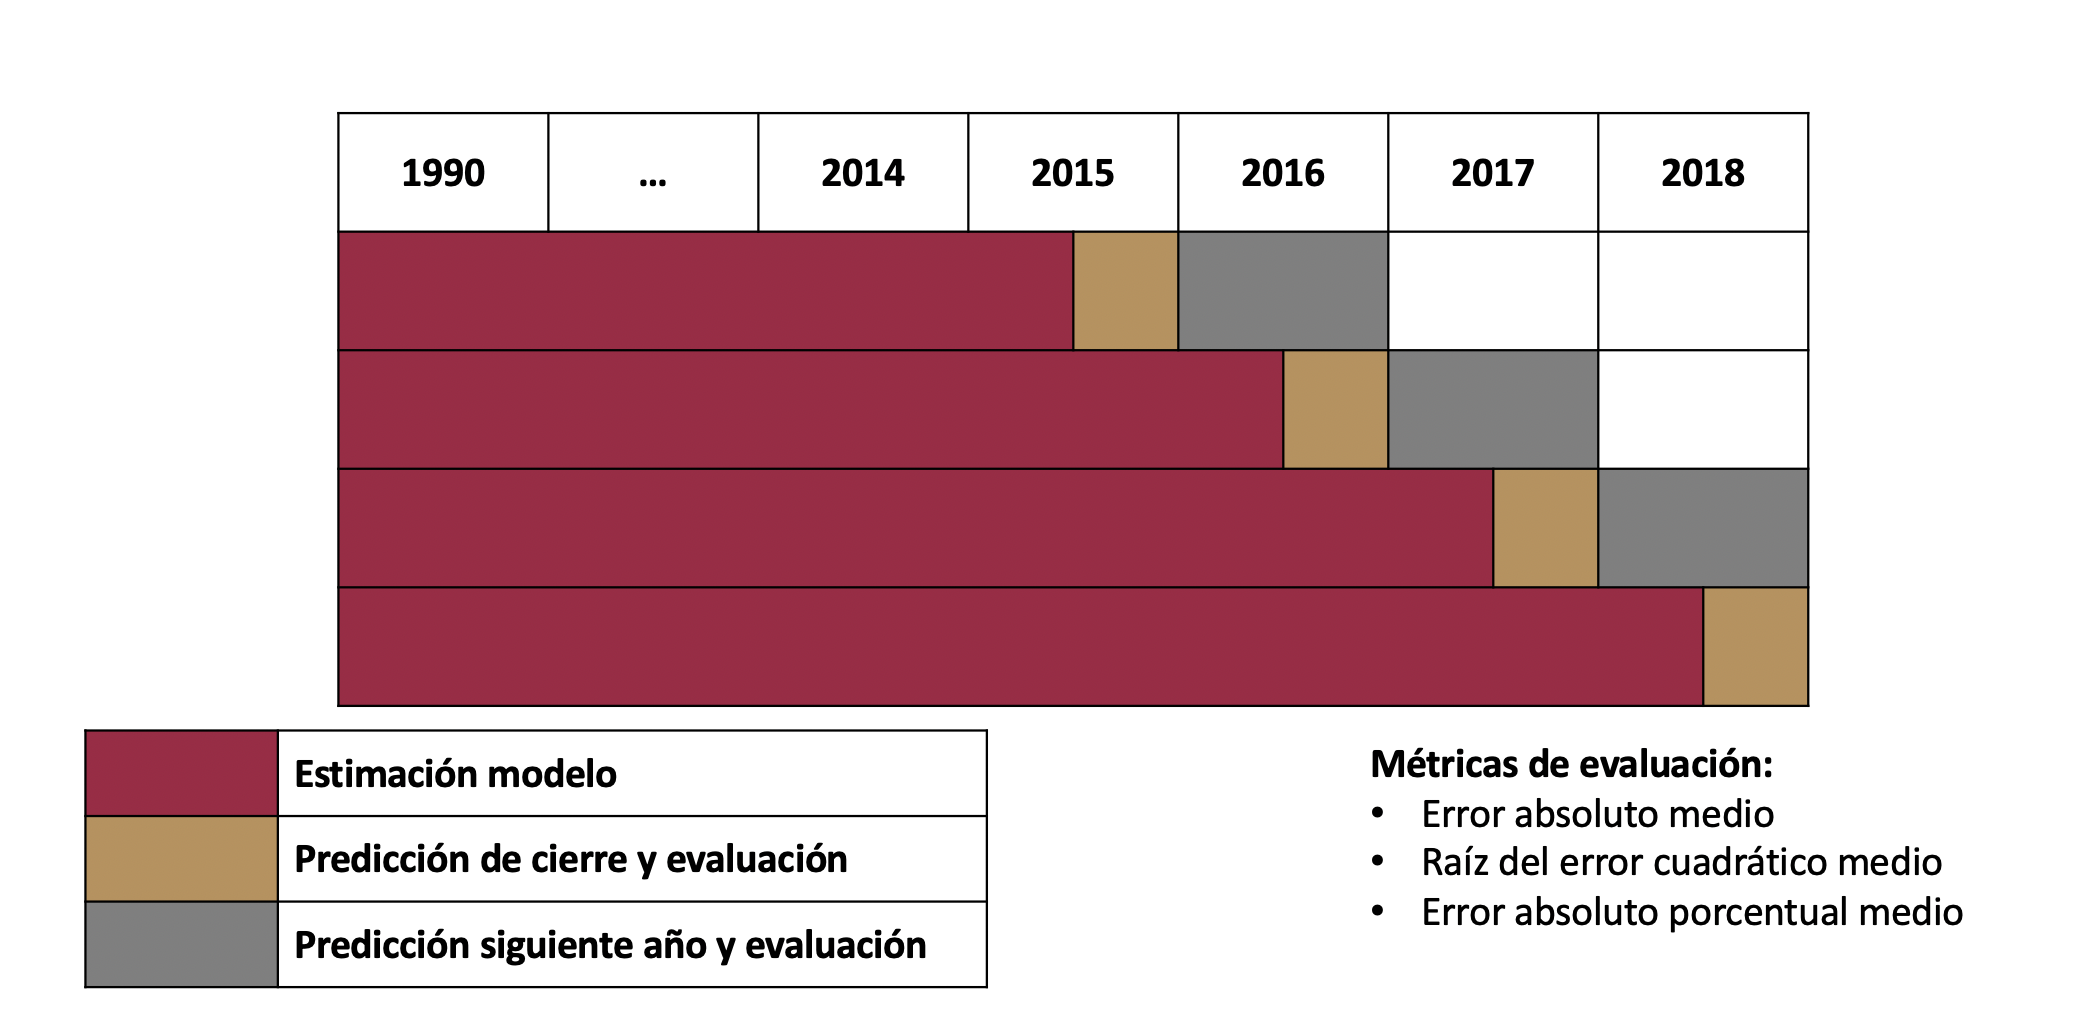
\includegraphics[scale = 0.3]{figures/cross_validation}
\end{figure}
Como se indica en la figura ~\ref{fig:cross_validation}, las métricas de evaluación que se construyeron fueron el error absoluto medio (Denominado MAE por \textit{Mean absolute error}), el error absoluto porcentual promedio (Conocido como MAPE por  \textit{Mean absolute percentual error}) ], y la raíz del error cuadrático medio (Denominado RMSE por \textit{Root mean squared error}). Ver ecuaciones ~\ref{eq:mae}, ~\ref{eq:mape} y ~\ref{eq:rmse} para definición formal.
\begin{align} 
mae &= (\sum_{t=1}^{n}{\left|\hat{y_{t}} - y_{t}\right|})\frac{1}{n} \label{eq:mae}\\
mape &= (\sum_{t=1}^{n}{\left|\hat{y_{t}} - y_{t}\right|\frac{1}{y_{t}}})\frac{1}{n} \label{eq:mape}\\
rmse &=\sqrt{(\sum_{t=1}^{n}{(\hat{y_{t}} - y_{t})^{2}})\frac{1}{n}} \label{eq:rmse}
\end{align}
Donde $\hat{y_{t}}$ es el valor predicho, $y_{t}$ es el valor observado, y $n$ es el número de periodos predicho.\\

Se priorizaron aquellos modelos que obtuvieron el menor \textit{rmse} y el menos \textit{mape} para la selección.
\subsection*{Modelos estimados}
En esta sección expondremos los modelos que seleccionamos para el ejercicio. Como breve introducción, nos enfocamos en tres modelos econométricos y tres modelos de Machine Learning. Los modelos econométricos fueron ARIMA, ARIMA con ajuste estacional (SARIMA) y Vectores Auto Regresivos. Seleccionamos los modelos  ARIMA y SARIMA porque son y han sido utilizados por la SHCP para predecir los ingresos tributarios mensuales. Gracias a esto, por un lado fuimos capaces de comparar los resultados de modelos alternativos con los modelos tradicionales, y por otro lado, dejamos un \textit{script} que puede ser reutilizado por la UPIT para continuar con las estimaciones tradicionales. El modelo de Vectores Auto Regresivos se seleccionó por ser uno de los modelos más utilizados para estimar relaciones macroeconómicas en las que un grupo de variables son endógenas entre sí. Es, por ejemplo, el modelo utilizado por (Capristán, et al. 2011) para estimar el impacto que tiene el tipo de cambio sobre la inflación, para lo cual modela un sistema de ecuaciones endógenas que incluyen el IGAE, el Tipo de Cambio, el Índice Nacional de Precios al Consumidor y la Tasa de Interés, utilizando variables exógenas similares a las que utilizamos aquí. \\

Los modelos de Machine Learning que se seleccionaron fueron, en primer lugar \textit{Decision Trees}, por ser uno de los modelos más sencillos y más fáciles de exponer. La facilidad de explicación es importante en un contexto de decisión de políticas públicas en el que el tomador de decisiones no es necesariamente es experto en modelación, como puede ser la aprobación de la Ley de Ingresos de la Federación. Los otros dos modelos: \textit{Random Forests} y \textit{Gradient Boosting} son ampliaciones del primer modelo, que aprovechan la estructura de los Árboles de Decisión para estimar cientos o miles de ellos y obtener modelos más robustos. Por compartir la misma estructura, y por ser de los modelos más utilizados de \textit{Machine Learning}  se optó por ellos. A continuación vemos una explicación con mayor detalle de los modelos seleccionados:

\begin{enumerate}
\item Modelos Auto Regresivos Integrados de media Móvil (ARIMA):\\

Los modelos ARIMA son modelo de una variable endógena definidos por tres parámetros $(p, d, q)$: Un componente auto regresivo ($p$), un componente de media móvil ($q$) y un grado de diferenciación de la variable para convertirla en estacionaria (Sabau, 2011). Los modelos ARIMA estiman la siguiente ecuación:

\begin{equation}
d(y_{t}, d) = \alpha_{0} + \sum_{i = 1}^{p}{\phi_{i}d(y_{t-i}, d) + \beta_{t}X_{t-i}} + \sum_{i = 1}^{q}{\theta_{i}\epsilon_{t-i}} + \epsilon_{t}
\end{equation}
Donde $d(y_{t}, d)$ es la diferencia $i$ de la variable endógena\\
$y_{t}$, $\alpha_{0}$, $\phi_{i}$ y $\theta_{i}$ son los parámetros a estimar de la variable endógena\\
$\beta_{t}$ es un vector de coeficientes de las variables exógenas $X_{t}$, y \\
$\epsilon_{t}$ es el error.

Para cada una de las variables endógenas se estimaron los parámetros auto regresivos del 1 al 6 y de media móvil del 1 al 6, resultando en 36 posibles combinaciones. En términos de las variables exógenas, se estimó una versión utilizando únicamente variables \textit{dummies} indicando los años 2009 y 2015, por la crisis financiera y la reforma tributaria de 2014, dummies de los meses de enero, marzo, abril y diciembre que tienen niveles de recaudación atípicamente altos, y series de los diferentes niveles de tasas de ISR a personas físicas, ISR a personas morales e IVA. Se estimó otra versión incluyendo al IGAE al grupo de variables exógenas, y otra versión incluyendo a todas las variables exógenas descritas en la parte inicial de esta sección.

\item Modelos Auto Regresivos Integrados de media Móvil con ajuste estacional (SARIMA):\\

Los modelos SARIMA son una extensión de los modelos ARIMA, que permiten incluir un componente estacional (Box and Jenkins, 1976). Estos modelos está definidos por siete parámetros $(p, d, q), (P, D, Q), s$. Los primeros tres representan lo mismo que los tres parámetros de los modelos ARIMA. El segundo grupo de tres representa los componentes estacionales, donde la $P$ representa el componente auto regresivo estacional, la $Q$ el componente de media móvil estacional, $D$ la diferencia de la variable estacional, y $s$ el número de periodos que componen un ciclo. Matemáticamente, estos modelos estiman la siguiente ecuación:

\begin{equation}
d(y_{t}, d) = \alpha_{0} + \sum_{i = 1}^{p}{\phi_{i}d(y_{t-i}, d) + \beta_{t}X_{t-i}} + \sum_{i = 1}^{q}{\theta_{i}\epsilon_{t-i}} + \varphi_{s}d(y_{t-s}, d) + \sum_{i = 1}^{P}{ \varphi_{s}\phi_{i}d(y_{t-s-i}, d)}+ \sum_{i = 1}^{Q}{ \varphi_{s}\theta_{i}\epsilon_{t-s-i}}+\epsilon_{t}
\end{equation}
Donde $\varphi_{s}$ es el coeficiente de estacionalidad y las demás variables representan lo mismo que en el modelo ARIMA.\\
Para cada una de las variables endógenas se estimaron los parámetros auto regresivos $p$ del 1 al 3, de media móvil $q$ del 1 al 3, con estacionalidad $s$ de 12, y componentes auto regresivos y de media móviles estacionales  $P$ y $Q$ del 1 al 2. Resultando en 36 posibles combinaciones también. En cuanto a las variables exógenas, al igual que con los modelos ARIMA, cada modelo se estimó con tres grupos de variables exógenas.

\item Vectores Auto Regresivos: \\
Los modelos de Vectores Auto Regresivos (VAR) tienen como objetivo de modelar un grupo variables endógenas entre sí. Son muy utilizados para estimar modelos macroconómicos estructurales, en los que por ejemplo, la tasa de interés, el tipo de cambio, la producción y los precios se determinan por las autocorelaciones de cada uno, y los rezagos de las demás variables. Son modelos que estiman un sistema de ecuaciones de la siguiente forma:
\begin{equation}
Y_{t} = \alpha_{0} + \sum_{i=1}^{L}{A_{i}Y_{t-i}} + \sum_{i=0}^{L}B X_{t-i} +E_{t}
\end{equation}
Donde $Y_t $ es un vector de variables endógenas\\
$X_{t}$ es un vector de variables exógenas\\
$A$ es un vector de coeficientes de las variables endógenas\\
$B$ es un vector de coeficientes de las variables exógenas\\
 $E_{t}$ es un vector de componentes de error.\\
 En los modelos VAR se selecciona el número de rezagos minimizando criterios de información que disminuyen al incrementar el poder explicativo del modelo pero penalizan por complejidad. Los más comunes son el criterio de información Akaike y el criterio de información Bayesiano, siendo el primero más laxo con la complejidad. Otro parámetro importante de los modelos VAR son si se estiman con una constante, o con una constante y una tendencia. En nuestras estimaciones, probamos con constante y con constante y tendencia, así como los rezagos indicados por ambos criterios de información. 

\item Árboles de decisión
Los árboles de decisión agrupan la información del set de información de entrenamiento en grupos de observaciones con la menor varianza posible en términos de la variable objetivo, y crean una serie de reglas para predecir información futura. En el caso más sencillo, que es el de predicción binaria, un árbol de decisión identifica las variables que logran una división más limpia de la información de manera recursiva. Para ejemplificar esto, sirve seguir el ejemplo presentado por (Provost y Fawcet, 2013) donde jugamos el rol de un banco que desea predecir los clientes que tienen más probabilidad de no pagar un crédito. Partimos de que contamos con una base de datos de 30 clientes de los cuales conocemos, además de si cayeron o no en impago, el balance que tenían en su cuenta bancaria y si contaban con casa propia o no. 
\begin{figure}[hbt!]
    \centering
     \caption{División con base en balance}
     \label{fig:dt_1}
     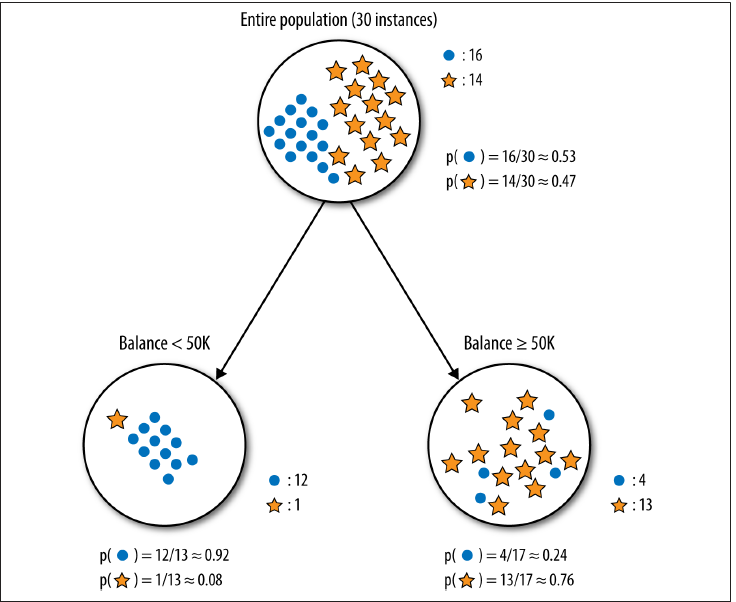
\includegraphics[scale = 0.6]{figures/dt_1}
\end{figure}
\begin{figure}[hbt!]
    \centering
     \caption{División con base en vivienda}
     \label{fig:dt_2}
     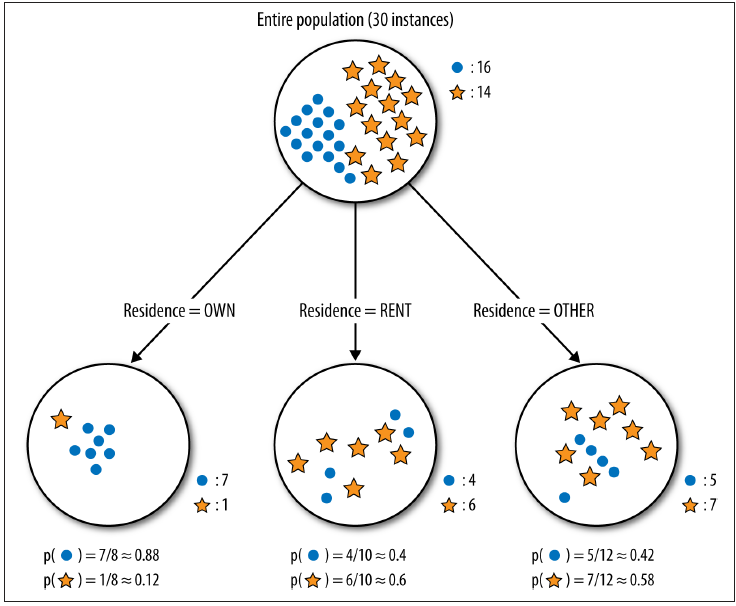
\includegraphics[scale = 0.6]{figures/dt_2}
\end{figure}

En la figura ~\ref{fig:dt_1} podemos ver lo que pasaría si dividimos las observaciones entre aquellas que tenían más o menos de 50 mil USD en el banco. El resultado son dos grupos que en promedio son más homogéneos que el grupo inicial de 30 observaciones. En la figura ~\ref{fig:dt_2}  vemos el resultado de dividir a las observaciones usando el criterio de tipo de propiedad. La homogeneidad también aumenta, sobre todo para el grupo que es propietario de un bien raíz, pero en promedio, la reducción en la heterogeneidad es mayor al usar el balance. Por lo tanto, el árbol de decisión escogería la variable de balance para hacer el primer nodo. De forma recursiva, este árbol continuaría dividiendo las ramas hasta que sean completamente puras (todas las observaciones en una rama tienen el mismo valor para la variable objetivo), hasta que se llegue a la profundidad máxima del árbol, o hasta que se llegue a un número mínimo que queremos que tengan las ramas. Todas las variables que limiten la profundidad de las ramas, sirven para controlar el \textit{overfitting}.

Algunos de los parámetros que se pueden especificar en un árbol de decisión de una variable continua son los siguientes:
\begin{enumerate}
\item Medida de heterogeneidad: Se puede escoger que heterogeneidad se mida con el error cuadrático medio, con el error absoluto promedio, o con una modificación al error cuadrático medio denominado \textit{friedman mse}
\item Profundidad máxima: Se puede especifica la profundad máxima que una rama puede tener. Para nuestras estimaciones, probamos con profundidades de 1,5,10,20,50 y 100.
\item Máximo número de variables a considerar: Cada \textit{split}, el árbol de decisión analiza un grupo de variables y encuentra la variable que logra la mejor división. Una forma de controlar el \textit{overfitting} es limitar el número de variables a analizar. Probamos árboles de decisión sin limitar, limitando con la raíz del número total de variables, y limitando con el logaritmo natural.
\item Mínimo número de observaciones para hacer split: Se puede especificar un número mínimo de observaciones que una rama necesita tener para que el árbol continúe haciendo divisiones. Probamos con 2, 5, y 10.
\end{enumerate}
\item \textit{Random Forests}
Los \textit{Random Forests} son un ensamble de muchos árboles de decisión, que al final se promedian entre sí para lograr una regla de decisión definitiva. Cada uno de los nodos de estos árboles es estimado usando un grupo aleatorio de las variables disponibles, el cual se elige con \textbf{reemplazo}, similar a las técnicas de \textit{bootstrapping}. Esto es lo que hace que los árboles no sea idénticos entre sí. Los \textit{Random Forests} disminuyen el \textit{overfitting} y al ser el promedio de número grande de árboles, potencialmente representan mejor a la población objetivo. El parámetros adicional más importante que los \textit{Random Forest} pueden tomar es el número de árboles a estimar. Nosotros probamos con 100 y 1000 árboles.

\item \textit{Gradient Boosting}
La técnica de \textit{Gradient Boosting} es también una técnica de ensamble, que estima un alto número de árboles de decisión y los promedia al final. La diferencia con \textit{Random Forests} es que los árboles se van estimando de tal forma que el peso de las observaciones en las que los árboles tienen peor desempeño se va incrementando. Es decir, se estima un árbol de decisión y se evalúa la precisión que habría tenido. Una vez identificadas las observaciones sobre las cuales el árbol habría tenido el mayor error, se incrementa el pesos de esas observaciones, y se estima un segundo árbol. Este proceso continúa sucesivamente hasta llegar al número máximo de árboles. Los principales parámetros adicionales que toman estos modelos son:
\begin{enumerate}
\item Número de árboles: Probamos con 100 y 1000.
\item Tasa de aprendizaje: Tasa a la cual se incrementa el peso de las observaciones mal predichas: probamos con 0.1 y 0.5
\item Muestra: Tamaño de la muestra para volver a estimar los árboles. El máximo valor es 1, indicando que siempre se utilice la totalidad de las observaciones. Probamos con 0.1, 0.5 y 1.
\end{enumerate}
\end{enumerate}

\subsection*{Modelos de variables exógenas}
Para utilizar modelos con variables exógenas en un contexto real, sería necesario predecir primero esas variable, y después incluirlas en el modelo. Por ejemplo, si se va a utilizar el IGAE para predecir los ingresos tributarios del siguiente año, sería necesario estimar el comportamiento del IGAE durante ese periodo. Para simular de mejor manera el contexto real, para cada corte de predicción estimamos las variables exógenas usando modelos predictivos en vez de tomar los valores observados. Específicamente, para cada corte estimamos un marco macroeconómico en dos pasos

\begin{enumerate}
\item En primer lugar, un modelo de las variables externas a México.
El primer modelo que estimamos fue uno para las variables externas a México. Estimamos un modelo VAR para las variables endógenas:
\begin{enumerate}
\item Índice de Producción Industrial de Estados Unidos
\item Índice de Precios al Consumidor de Estados Unidos
\item Tasa de interés promedio mensual de los bonos del tesoro de Estados Unidos con vencimiento trimestral.
\item Índice del tipo de cambio del dólar de Estados Unidos contra el resto de las monedas del mundo, ponderado por el nivel de comercio.
\item Índice de precios de las Materias Primas.
\end{enumerate}
Como variables exógena incluimos dos dummies, una para el año 2000 y otra para el 2009, reflejando las crisis financieras de esos años.\\
Las variables endógenas las incluimos en la diferencia de sus logaritmos, para transformarlas en estacionarias. El número de rezagos se seleccionó con el criterio de información Bayesiano, e. cual únicindicó únicamente 1 rezago. Se escogió este criterio porque tuve una precisión mayor para predecir el Índice de Producción Industrial de Estados Unidos que el criterio Akaike.

\item Modelo del marco macroeconómico de México
Una vez que tuvimos predicciones para las variables de Estados Unidos, realizamos predicciones para el Marco Macroeconómico de México. En este modelo, incluimos las siguientes variables endogenas:
\begin{enumerate}
\item IGAE con ajuste estacional
\item Tasa de interés de CETES con vencimiento a 91 días.
\item Tipo de cambio mensual
\item Índice Nacional de Precios al Consumidor
\item Flujo mensual de importaciones en pesos
\item Indicador mensual de consumo
\item Ingresos del sector público netos
\end{enumerate}
La lógica de incluir a los ingresos del sector público en su valor total es que estos son determinantes del gasto público, y además de depender del resto de las variables macroeconómicas, son determinantes del crecimiento económico. Además, este modelo VAR es uno de los dos mejores modelos predictivos de los ingresos tributarios, como veremos en los resultados. El modelo se estimó con 12 rezagos, que fue lo indicado por el criterio de Información Akaike, el cual dio mejores resultados en las estimaciones históricas que el criterio Bayesiano.\\

Como variables exógenas, incluimos las variables que estimamos en el VAR de variables externas, además de una dummie para indicar la crísis de 2009, y dummies para indicar el mes en el que cayó Semana Santa de cada año. Las variables las incluimos en las primeras diferencias de sus logaritmos. 

De acuerdo con la última estimación, pronosticamos lo siguiente:
\begin{enumerate}
\item Crecimiento modesto de la economía mexicana de 0.3\% en 2019.
\item Depreciación del tipo de cambio promedio de 0.2\%.
\item Inflación de 3.6\%
\item incremento e la tasa de CETES de 3.1\%  (incremento de 20 puntos base)
\item (disminución de las importaciones en pesos en 4.2\%
\item incremento en los ingresos tributarios de 8.5\%.
\end{enumerate}

\end{enumerate}


\subsection*{Mismos modelos con diferentes grupos de variables endógenas}
Los modelos que permitne más de una variable endógena, como el VAR o los modelos de Machine Learning, los estimamos probando diferentes grupos. En el caso del VAR es un procedimiento sencillo, pues el número de variables que se incluyen determina el número de ecuaciones que se estiman. En el caso de los modelos de Machine Learning, incluir más de una variable endógena significa incluir a todas las variables en el vector de variables a predecir, y crear variables dummies que indican cuál es la variable endógena que se va a predecir. Por ejemplo, si se incluye IVA e ISR en las variables endógenas, se agregaría una dummie a la lista de variables exógenas que indicará si se esta prediciendo IVA o si se está prediciendo ISR.

\subsection*{Método de predicción recursivo}
Finalmente, es importante destacar que se siguió un método de predicción recursivo para todos los modelos. En este enfoque, cada observación que se predice, sirve como rezago para predecir la siguiente observación. En el caso de los modelos econométricos, este es el enfoque tradicional y es el comportamiento que siguen los paquetes estadísticos. En el caso de \textit{Machine Learning} existen dos enfoques principales. Uno es este, en el que se entrena únicamente un modelo para predecir la siguiente observación, y el mismo modelo es aplicado recursivamente hasta completar todas las observaciones que se buscan predecir. Otro enfoque, es entrenar un modelo para cada uno de las observaciones a predecir. Es decir, se entrena un modelo que predice la observación inmediata, otro que predice aquella observación a dos observaciones de distancia, y así sucesivamente hasta cubrir todos los pasos. Elegimos el enfoque recursivo por varias razones: es más similar al econométrico, lo cual hace más comparables ambos enfoques, y es menos costoso computacionalmente, pues en vez de entrenar 12 modelos para predecir los meses de un año, se entrena uno solo.

\section*{Resultados}

En total se realizaron 21,468 estimaciones. Estas son el resultado de 4 periodos de predicción, 5 variables a predecir, 6 enfoques y múltiples combinaciones de parámetros para cada modelo. De estos, ARIMA  fueron 1651, SARIMA 2608, VAR 1008, Árboles de Decisión 9720, \textit{Random Forests} 3844 y \textit{Gradient Boosting} 2637. Para cada una de estas estimaciones obtuvimos la calidad de la predicción para el periodo de cierre (los siguientes 6 meses), para el periodo completo de 18 meses y para el periodo de 12 meses del siguiente año.\\

La selección de los mejores modelos es sensible a la medida de precisión que se utilice. Si buscamos los mejores modelos para predecir el cierre del año en curso, el grupo de mejores modelos es ligeramente distinto al que se obtiene si maximizamos la precisión del periodo completo de predicción (18 meses). \\

En la tabla ~\ref{tab:best_models} presentamos el mejor modelo para cada variable de acuerdo con el horizonte de predicción que prioricemos, así como las medidas de precisión asociadas. Comenzando con los ingresos tributarios, el mejor modelo para los horizontes de predicción de 18 meses y de los 12 meses del siguiente año es un ARIMA de órden (3, 0, 3) con las variables  exógenas que se listan en la nota al pie número 3. Esto modelo logró en promedio un error porcentual promedio en los primeros seis meses de predicción de 7\%, de 8\% en el periodo completo y de 9\% en el año siguiente. En términos de la raíz del error cuadrático promedio, en los primeros seis meses es de 19,565 MDP por periodo, de 26,550 MDP para el siguiente año y de 24,224 MDP para el periodo completo. En estos resultados empezamos a notar que 7\% de error promedio para cifras como los ingresos tributarios, equivale a cantidades relevantes para gobierno. Continuando con los ingresos tributarios, si maximizamos el cierre del año, el mejor modelo es un SARIMA (2, 0, 3)(1, 0, 1, 12) con las mismas variables exógenas que el anterior, el cual logró una error porcentual promedio de 4\% los meses del cierre.\\

Siguiendo con los ingresos tributarios sin contar a los IEPS a la gasolina, el mejor modelo según los horizontes 18 meses y 12 meses del siguiente año es un ARIMA de órden (4, 0, 5) con las variables exógenas que se indican en el pie de tabla 1. El error porcentual promedio es de 6\% para todos los horizontes de predicción. El modelo que mejor se desempeñó para predecir el cierre es un SARIMA (3, 0, 3)(1, 0, 1, 12), que logró 5\% de error porcentual promedio.  Si seguimos viendo la tabla, vemos que los mejores modelos para predecir el ISR son un VAR con variables endógenas de ISR y de impuesto a las importaciones para el periodo completo y para el siguiente año, y un SARIMA (2, 0, 3)(1, 0, 0, 12) para el cierre del año. Vemos que la precisión de los modelos predictivos de ISR fue de 5\% para predecir el cierre, y de 6\% y 7\% para predecir 18 meses y el siguiente año.\\

En el IVA vemos una capacidad predictiva mucho menor que en las variables que hemos revisado. El error porcentual promedio está casi siempre por encima del 10\%. Resalta que el mejor modelo para los tres horizontes es un SARIMA, aunque cada uno con diferente especificación. Para el impuesto a las importaciones, los modelos de \textit{Machine Learning} tuvieron mejor desempeño que los econométricos. Para cierre y el siguiente año, el mejor modelo es un \textit{Gradient Boosting}, que logró un error porcentual promedio de 5\% y de 11\% respectivamente. Sin embargo, para el periodo completo, el que mejor se desempeñó fue un Random Forests, con 10\%. Es notable que el impuesto a las importaciones es el único caso en el que el mejor modelo es de \textit{Machine Learning}. Finalmente, para el IEPS a productos diferentes a la gasolina la precisión es muy baja. Casi siempre al rededor de 18\%, suficientemente baja para no explorar a profundidad.\\

Para poner en contexto estos resultados, presentamos la precisión que ha tenido el Calendario de la Ley de Ingresos de la Federación desde 2015 hasta 2019 en la table \ref{tab:lif}. Los resultados que vemos son el promedio del error porcentual promedio y  la raíz del error cuadrático medio en los años de 2016 a 2018 para los ingresos tributarios, el IVA, el ISR, el IEPS y el impuesto a las importaciones. Vemos que el error porcentual ha sido de 6\% para los ingresos tributarios, de 7\% para el ISR, de 10\% para el IVA,  de 17\% para el IEPS y 18\% para el impuesto a las importaciones. Para ser totalmente justos, esas cifras las vamos a comparar con el error porcentual promedio de los 12 meses del siguiente año, pues el calendario se realiza desde enero y sería injusto compararlo con la precisión con la que podemos estimar el cierre del año. En los ingresos tributarios la LIF en promedio ha logrado mayor precisión, pues han sido de 6\% contra 9\% de nuestro mejor modelo. En ISR nuestras estimaciónes  han sido ligeramente superiores, con 6\% de precisión contra 7\% de la LIF. En IVA hemos logrado la misma precisión de 10\% y en el impuesto a las importaciones nuestros modelos han sido superiores. Es decir, hemos logrado resultados similares.\\

Para seguir siendo justos con la LIF, nosotros contamos con más información para seleccionar el mejor modelo que los funcionarios que hicieron la LIF de 2016, de 2017 y de 2018, lo cual nos colocó en una posición de ventaja. Sin embargo, para ser justos con nosotros, está en los mayores intereses del SAT lograr que la Ley de Ingresos se cumpla, y han contado con las herramientas necesarias para influir en los resultados. Recordemos que estamos hablando de recaudación neta, que es el resultado de restar de la recaudación bruta, las compensaciones y devoluciones. Estas dos han sido la llave que el SAT ha podido aflojar y apretar para que el flujo de ingresos se acerque a la Ley. En otras palabras, el calendario de la Ley de Ingresos lleva consigo un imán que atrae a los ingresos observados hacia ella. Por esta razón resaltamos en una de las cuatro conclusiones que la predicción de ingresos netos es una tarea compleja. Y como pudimos ver en los resultados de nuestros mejores modelos, hay impuestos que son menos predecibles que otros, como el IVA, en donde las compensaciones y devoluciones influyen más en los niveles mensuales de recaudación.

\begin{landscape}
\hspace{-3cm}
% Table generated by Excel2LaTeX from sheet 'best_for_each'
\begin{longtable}{p{3em}p{3em}p{5em}p{7em}p{2em}p{2em}p{2em}p{2em}p{2em}p{2em}p{2em}p{2em}p{2em}}
\caption{\label{tab:best_models}Mejores modelos para cada variable según RMSE de horizonte}\\
variable & \multicolumn{1}{l}{horizon} & model & params & endog & exog & \multicolumn{1}{l}{mapefirst6} & \multicolumn{1}{l}{mapefirst18} & \multicolumn{1}{l}{mapelast12} & \multicolumn{1}{l}{rmsefirst6} & \multicolumn{1}{l}{rmselast12} & \multicolumn{1}{l}{rmsefirst18} \\
\hline \hline
Ing. trib. & \multicolumn{1}{l}{12, 18} & ARIMA & (3, 0, 3) & -     & 3*    & 0.07  & 0.08  & 0.09  & 19656.34 & 26550.18 & 24226.09\\
Ing. trib. & 6     & SARIMA & (2, 0, 3),(1, 0, 1, 12) & -     & 3*    & 0.04  & 0.08  & 0.10  & 12165.67 & 31502.95 & 26481.73\\
\hline
Ing. trib. sin gas & \multicolumn{1}{l}{12, 18} & ARIMA & (4, 0, 5) & -     & 1*    & 0.06  & 0.06  & 0.06  & 15326.36 & 16866.31 & 16386.63\\
Ing. trib. sin gas & 6     & SARIMA & (3, 0, 3),(1, 0, 1, 12) & -     & 3*    & 0.05  & 0.07  & 0.08  & 12620.62 & 24171.51 & 20927.59\\
\hline
ISR   & \multicolumn{1}{l}{12, 18} & VAR   & ic: aic, maxlags: 12, trend: c & a*    & 3*    & 0.06  & 0.06  & 0.07  & 9201.59 & 13365.20 & 11958.91\\
ISR   & 6     & SARIMA & (2, 0, 3),(1, 0, 0, 12) & -     & 3*    & 0.05  & 0.09  & 0.12  & 6820.87 & 19672.15 & 16223.43\\
\hline
IVA   & 12    & SARIMA & (2, 0, 1),(1, 0, 0, 12) & -     & 3*    & 0.13  & 0.11  & 0.10  & 10391.88 & 8372.88 & 9163.58\\
IVA   & 18    & SARIMA & (2, 0, 1),(1, 0, 1, 12) & -     & 3*    & 0.13  & 0.11  & 0.09  & 10065.17 & 8413.28 & 9034.53\\
IVA   & 6     & SARIMA & (3, 0, 2),(1, 0, 0, 12) & -     & 1*    & 0.12  & 0.12  & 0.12  & 9630.61 & 10766.99 & 10349.82\\
\hline
Imps. importaciones & 12    & GB    & learningrate: 0.1, maxdepth: 10, nestimators: 1,, subsample: 0.5 & b*    & 4*    & 0.08  & 0.10  & 0.11  & 554.73 & 642.67 & 618.37\\
Imps. importaciones & 18    & RF    & criterion: mse, maxdepth: 5, maxfeatures: log2, minsamplessplit: 2, nestimators: 100,  & -     & 4*    & 0.07  & 0.10  & 0.11  & 453.37 & 674.80 & 618.11\\
Imps. importaciones & 6     & GB    & learningrate: 0.5, maxdepth: 1, nestimators: 50,, subsample: 1.0 & -     & 4*    & 0.05  & 0.14  & 0.20  & 312.67 & 1146.87 & 919.78\\
\hline
IEPS no gas & 12    & ARIMA & (4, 0, 5) & -     & 2*    & 0.19  & 0.18  & 0.18  & 2692.96 & 2562.04 & 2629.44\\
IEPS no gas & 18    & ARIMA & (5, 0, 1) & -     & 2*    & 0.18  & 0.18  & 0.18  & 2526.30 & 2638.72 & 2608.73\\
IEPS no gas & 6     & VAR   & ic: aic, maxlags: 12, trend: ct & c*    & 3*    & 0.11  & 0.19  & 0.22  & 2046.36 & 3891.99 & 3421.22\\
\hline \hline
\end{longtable}%
\noindent
1*	mes1, mes3, mes4, mes12, year2009, year2015, semanasanta, IVA, ISRP, ISRE, 
2*	igae, mes1, mes3, mes4, mes12, year2009, year2015, semanasanta, IVA, ISRP, ISRE, 
3*	igae, inpc, tasacetes91mensual, tcmensual, commoditypriceindex, importacionesr, indicmensconsumo, mes1, mes3, mes4, mes12, year2009, year2015, semanasanta, IVA, ISRP, ISRE, 
4*	all \\
\noindent
a*	ISR, Imps. importaciones, 
b*	ISR, IVA, Imps. importaciones, 
c*	ISR, IVA, IEPS no gas, Imps. importaciones, 
-	Sólo 1 variable endógena, 
\end{landscape}
 
% Table generated by Excel2LaTeX from sheet 'Promedio LIF'
\begin{longtable}{crr}
\caption{\label{tab:lif}Precisión promedio del Calendario de la Ley de Ingresos de la Federación de 2016 al 2019}\\
\textbf{variable} & \multicolumn{1}{c}{\textbf{mape}} & \multicolumn{1}{c}{\textbf{rmse}} \\ \hline \hline
Ingresos tributarios & 0.06  & 19124.45 \\ \hline
ISR   & 0.07  & 15247.59 \\ \hline
IVA   & 0.10  & 8784.10 \\ \hline
IEPS  & 0.17  & 6324.99 \\ \hline
Imp. Importaciones & 0.18  & 1084.30 \\ \hline \hline
\end{longtable}%

\subsection*{Estimando cierre}
Ahora nos enfocaremos en los resultados de las estimaciones de cierre. Recordemos que los datos de precisión que hemos visto hasta ahora han sido datos promedio. Cada uno de los modelos se estimó para predecir 18 meses a partir de cuatro cortes transversales: junio de 2015, 2016, 2017 y 2018. A continuación presentaremos los el error porcentual promedio de la mejor especificación de cada modelo para las variables de ingresos tributarios, ISR, IVA e impuesto a las importaciones. La selección de los mejores modelos de estas gráficas se realizó con base en el \textit{RMSE} de cierre, y las variables se seleccionaron por con fines ilustrativos y de importancia en la recaudación.\\
En la figura \ref{fig:ing_trib} podemos ver el error porcentual promedio de las predicciones realizadas de ingresos tributarios en cada corte transversal. El eje vertical está invertido, pues menor error porcentual significa mayor precisión. Es claro como el SARIMA tiene el mejor desempeño para todos los cortes, con excepción del último donde un modelo ARIMA lo supera. La precisión del mejor modelo se mantiene en un rango relativamente constante, entre 4 y 5.5\% aproximadamente, lo cual arroja confianza para las estimaciones. 
\begin{figure}[hbt!]
    \centering
     \caption{Ingresos tributarios}
     \label{fig:ing_trib}
     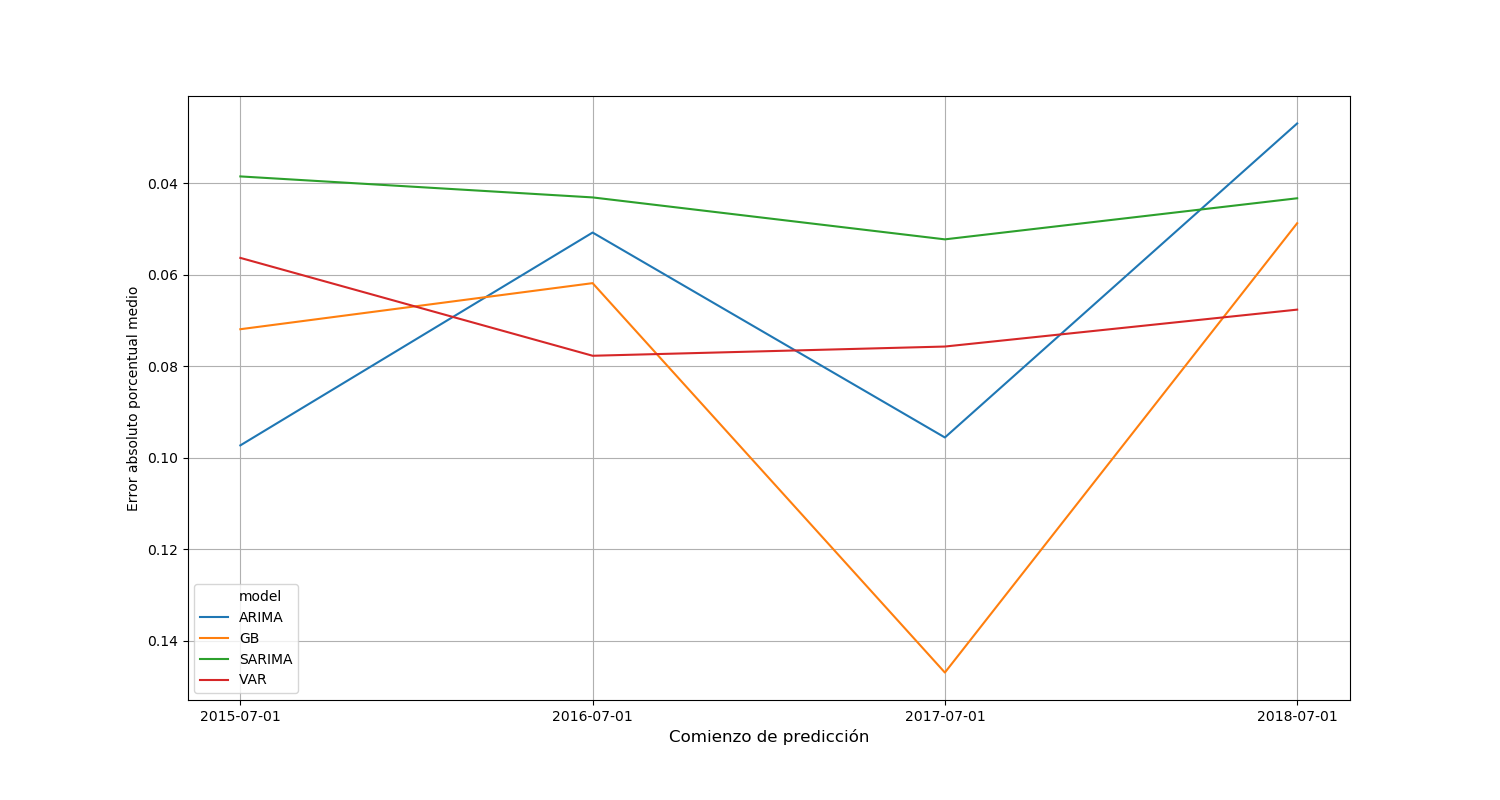
\includegraphics[scale = 0.4]{figures/ing_trib_neto_(mdp)_r_prec_cierre}
     \small\textsuperscript{a=} SARIMA (2, 0, 3)(1, 0, 1, 12) con variables economía mexicana y Estados Unidos, ARIMA(4, 0, 2) con variables exógenas de economía mexicana y Estados Unidos, VAR(criterio: Bayesiano, lags máximos: 12, constante sin tendencia, con variables endógenas economía mexicana y exógenas Estados Unidos
\end{figure}


En la figura \ref{fig:isr} presentamos el ISR. Se ve que el SARIMA no tuvo el mejor desempeño siempre, pues en los primeros dos cortes un modelo de árboles de decisión, un modelo ARIMA y un VAR tuvieron mejor desempeño. Sin embargo, para los últimos dos periodos de predicción, el SARIMA tuvo los mejores resultados. La predicción de este modelo se acerca al 2\% para el corte de 2018, después de haber estado en 3\% para el 2017. Por la cercanía de los resultados de SARIMA con VAR, será interesante estimar también un modelo VAR  y obtener dos predicciones.

\begin{figure}[hbt!]
    \centering
     \caption{ISR}
     \label{fig:isr}
     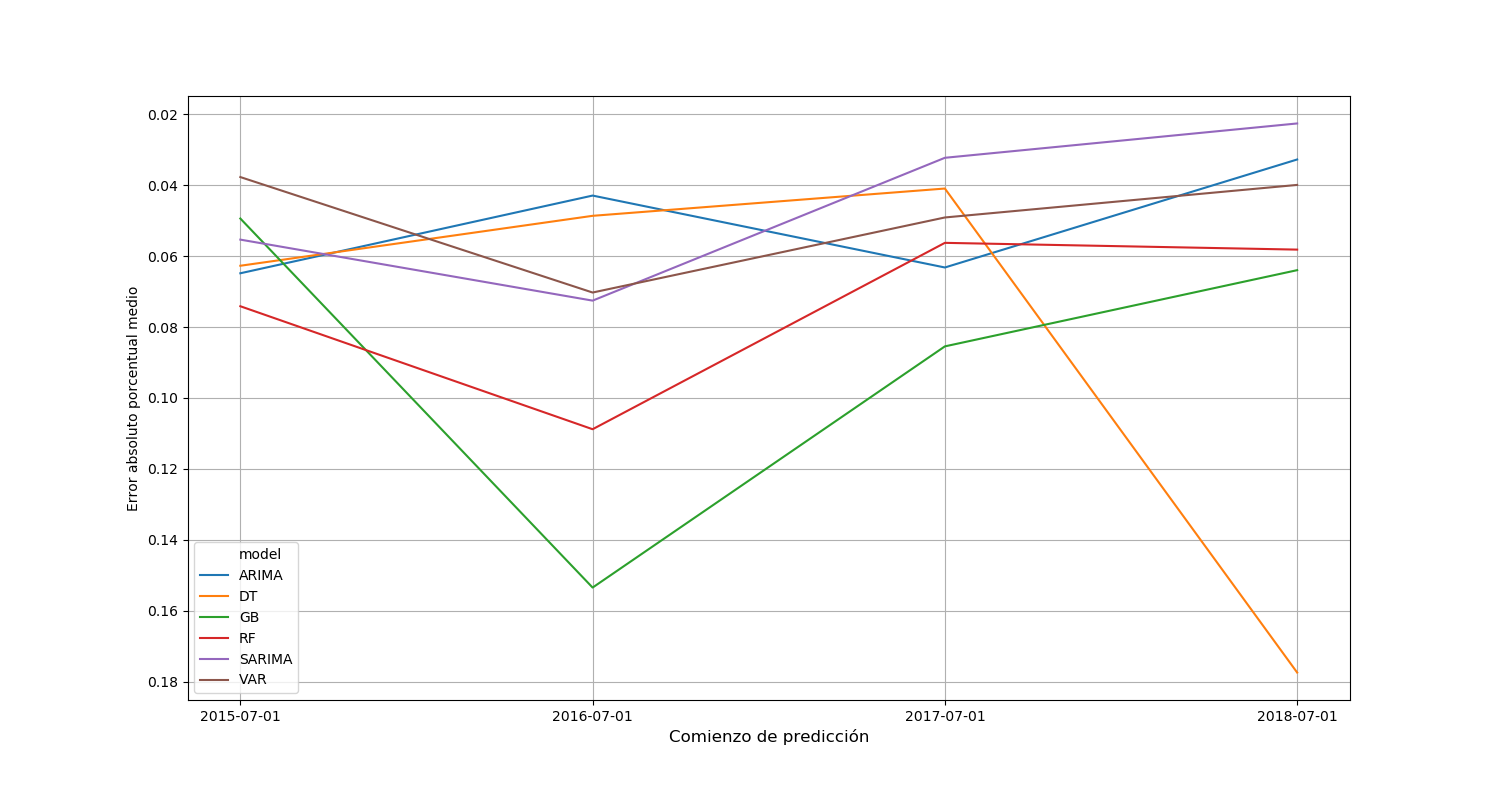
\includegraphics[scale = 0.4]{figures/isr_neto_(mdp)_r_prec_cierre}
      \small\textsuperscript{a=} SARIMA (2, 0, 3)(1, 0, 0, 12) con variables economía mexicana y Estados Unidos, ARIMA(1, 0, 4) con dummies de meses y tasas, VAR(criterio: Bayesiano, lags máximos: 12, constante sin tendencia, con variables endógenas Impuesto a las importaciones y exógenas de economía mexicana y Estados Unidos,  'RF (criterion': 'mse', 'max depth': 50, 'max features': 'log2', 'min samples split': 2, 'n estimators': 100), GB (learning rate': 0.1, 'max depth': 5, 'n estimators': 50),  DT(criterion': 'mae', 'max depth': 5, 'max features': 'log2', 'min samples split': 2)
\end{figure}

El IVA, en la figura  \ref{fig:iva} muestra un primer resultado claro. En 2017 el comportamiento fue atípico. Todos los modelos se desempeñaron peor de lo que venían logrando, llegando a errores porcentuales superiores al 14\%. Si bien el SARIMA es el modelo que en promedio obtiene los mejores resultados, no hay un claro modelo superior. Por su consistencia, el modelo de \textit{Random Forests} puede aportar predicciones útiles.\\

\begin{figure}[hbt!]
    \centering
     \caption{IVA}
     \label{fig:iva}
     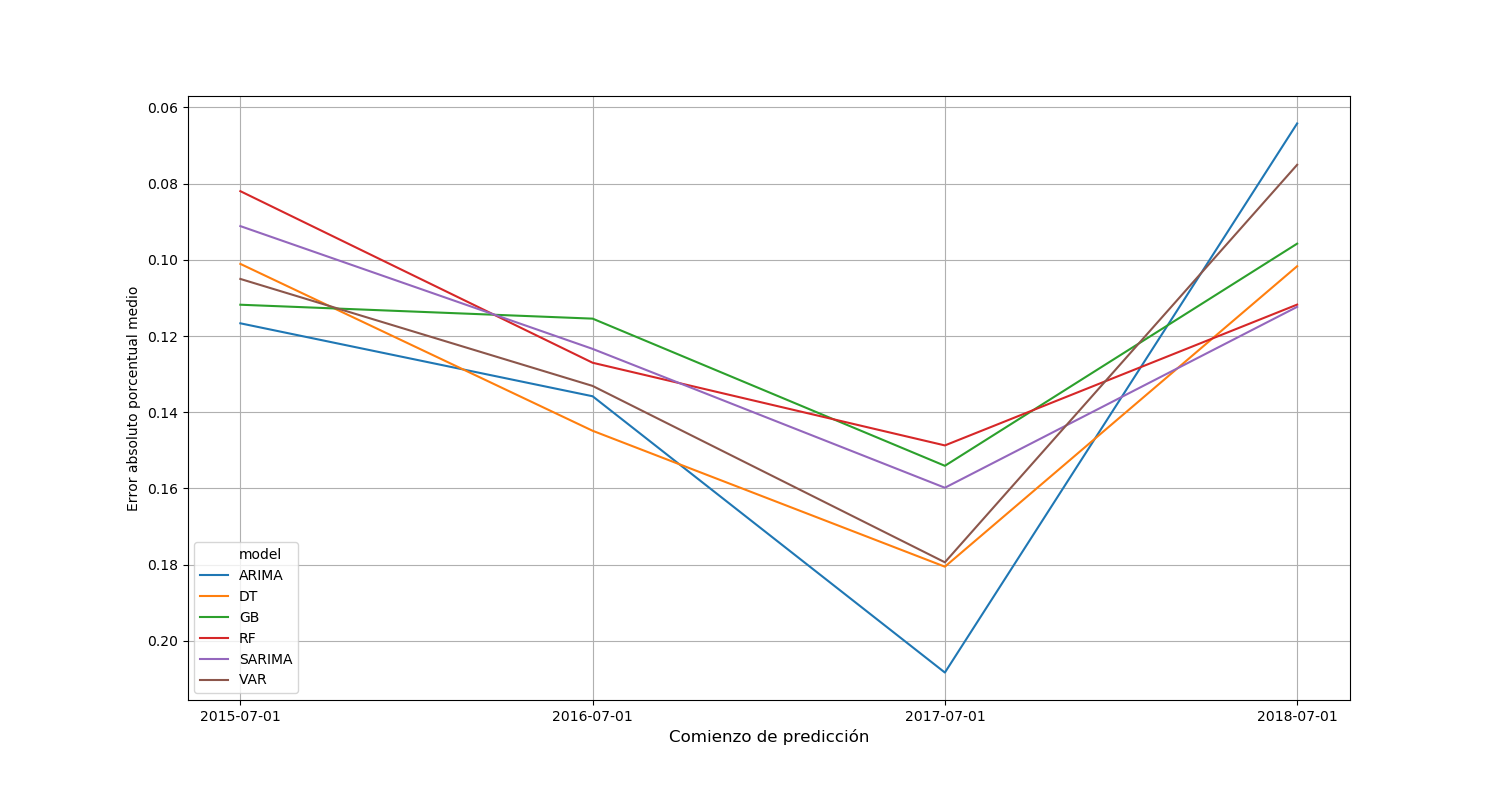
\includegraphics[scale = 0.4]{figures/iva_neto_(mdp)_r_prec_cierre}
      \small\textsuperscript{a=} SARIMA (3, 0, 2)(1, 0, 0, 12) con dummies de meses y tasas, ARIMA(5, 0, 5) con dummies de meses y tasas, VAR(criterio: Akaike, lags máximos: 12, constante sin tendencia, con variables endógenas Impuestos y exógenas de economía mexicana y Estados Unidos,  'RF (criterion': 'mae', 'max depth': 50, 'max features': 'sqrt', 'min samples split': 10, 'n estimators': 10), GB (learning rate': 0.1, 'max depth': 10, 'n estimators': 1, 'random state': 1234, 'subsample': 0.1),  DT(criterion': 'mae', 'max depth': 1, 'max features': 'log2', 'min samples split': 5)
\end{figure}

Finalmente, en la figura \ref{fig:imps} del impuesto a las importaciones vemos que el modelo SARIMA se desempeño bien para el tercer corte, y fue incrementando su precisión, sin embargo, para el último corte arrojó resultados muy inferiores. \textit{Random Forests} y \textit{Gradient Boosting} tuvieron un error porcentual promedio con menor varianza, entre 4\% y poco más de 6\%. 

\begin{figure}[hbt!]
    \centering
     \caption{Impuesto a las importaciones}
     \label{fig:imps}
     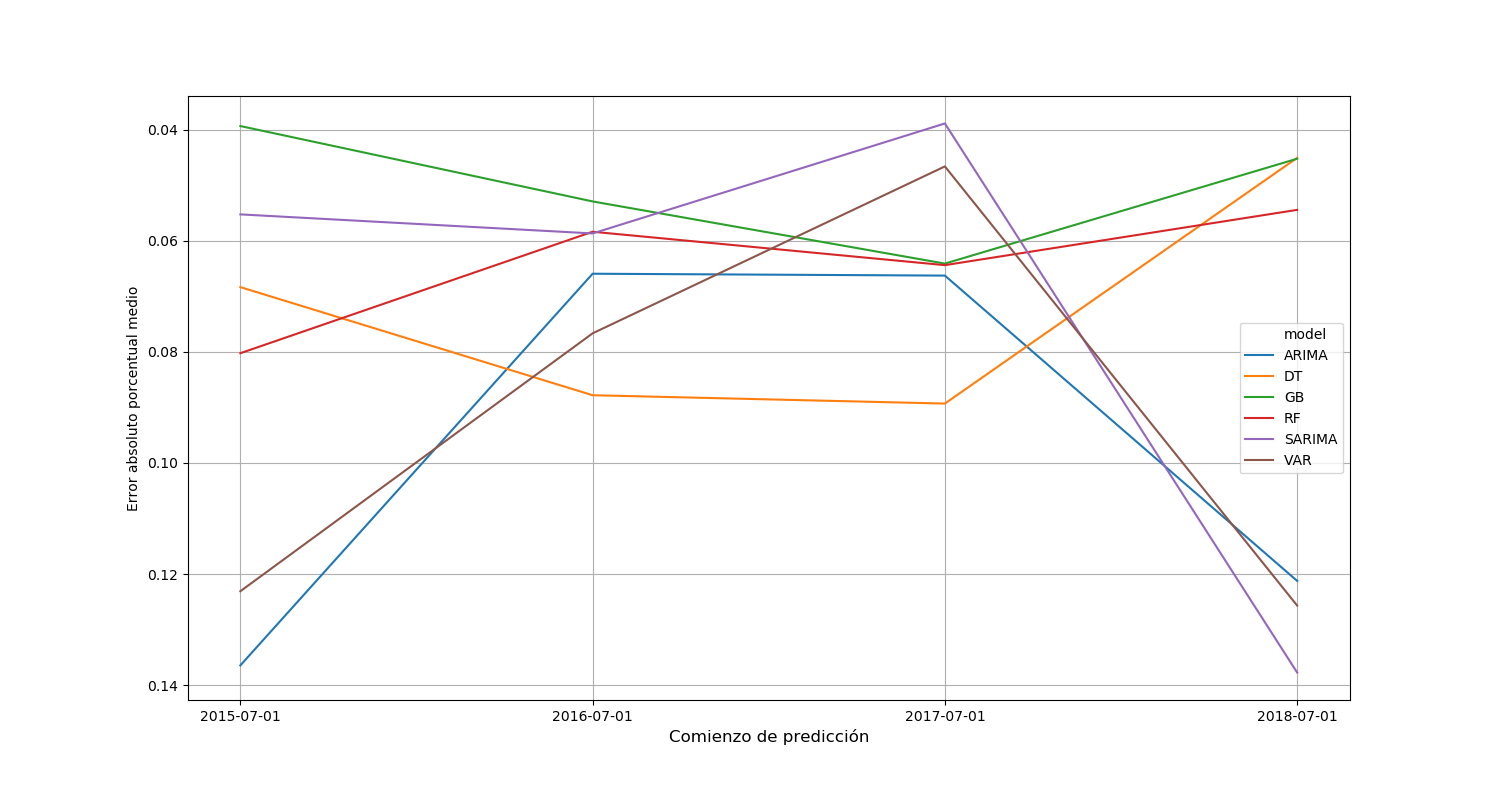
\includegraphics[scale = 0.4]{figures/importaciones_neto_(mdp)_r_prec_cierre}
      \small\textsuperscript{a=} SARIMA (3, 0, 3)(1, 0, 0, 12) con dummies de meses y tasas, ARIMA(4, 0, 5) con dummies de meses y tasas, VAR(criterio: Akaike, lags máximos: 12, constante sin tendencia, con variables endógenas Impuestos y exógenas de economía mexicana y Estados Unidos,  'RF (criterion': 'mse', 'max depth': 50, 'max features': 'sqrt', 'min samples split': 2, 'n estimators': 1000), GB ( learning rate': 0.5, 'max depth': 1, 'n estimators': 50),  DT(criterion': 'mse', 'max depth': 10, 'max features': None, 'min samples split': 2)     
\end{figure}
\newpage
\newpage
\FloatBarrier

\section*{Predicciones}
Una vez seleccionados los modelos, realizamos las predicciones para los impuestos analizados. Primero se realizaron predicciones mensuales, con principal énfasis en el cierre del año. En la figura \ref{fig:pred_ing_trib} podemos ver las predicciones anuales de los ingresos tributarios y los ingresos tributarios sin gasolina. En la figura \ref{fig:pred_isr_iva} podemos ver las predicciones de ISR y de IVA, y en la figura \ref{fig:pred_imp_ieps} las de IEPS sin gasolina y de importaciones. En el caso de ingresos tributarios totales, al haber sido el SARIMA claramente el mejor modelo, solo producimos predicciones con ese modelo. Sabemos que en pasadas ocasiones el error ha sido de aproximadamente 6\%.\\
Tanto para ISR como para IVA generamos dos predicciones. Para ISR una con un modelo SARIMA y otra con un modelo VAR en el que la otra variable endógena fueron los impuestos a las importaciones. En el caso del IVA, usamos el modelo SARIMA seleccionado, así como el de \textit{Random Forests}.\\
Finalmente, para el impuesto a las importaciones presentamos los resultados de \textit{Gradient Boosting} y para el IEPS sin gasolina, los resultados del modelo VAR y el modelo ARIMA. Se ve como para este último impuesto, ambos modelos dan resultados bastante diferentes.

\begin{figure}[hbt!]
    \centering
     \caption{Ingresos tributarios con y sin IEPS a las gasolinas}
     \label{fig:pred_ing_trib}
     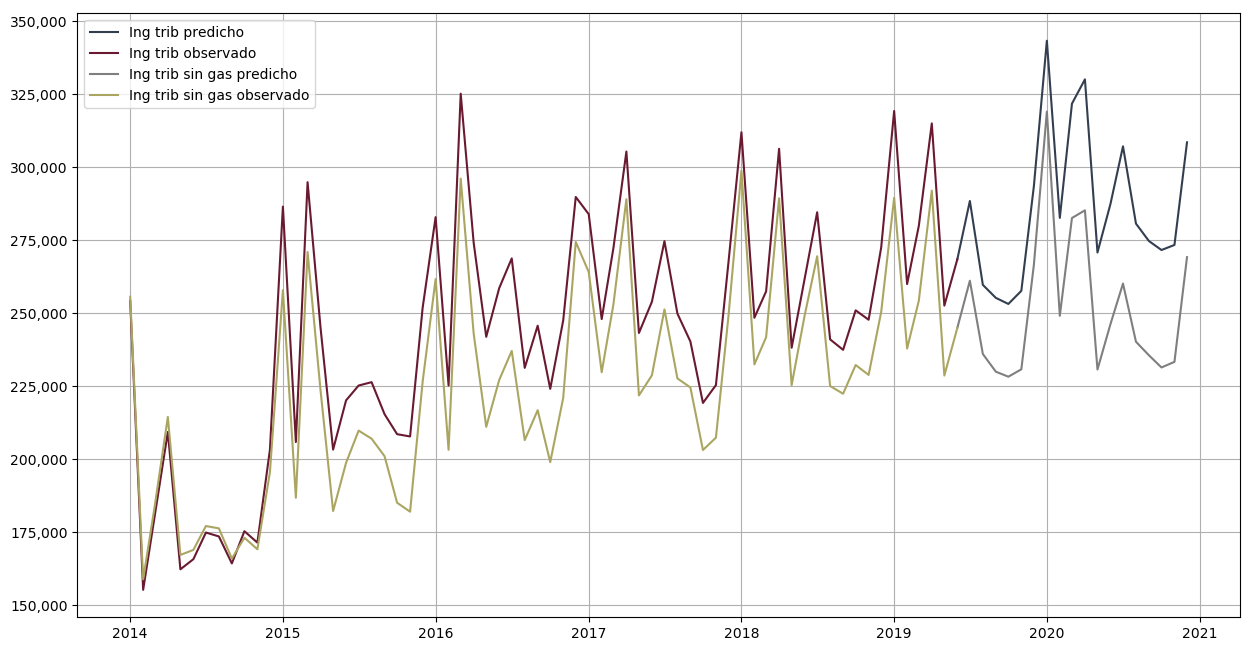
\includegraphics[scale = 0.5]{figures/pred_ing_trib}
\end{figure}

\begin{figure}[hbt!]
    \centering
     \caption{ISR e IVA}
     \label{fig:pred_isr_iva}
     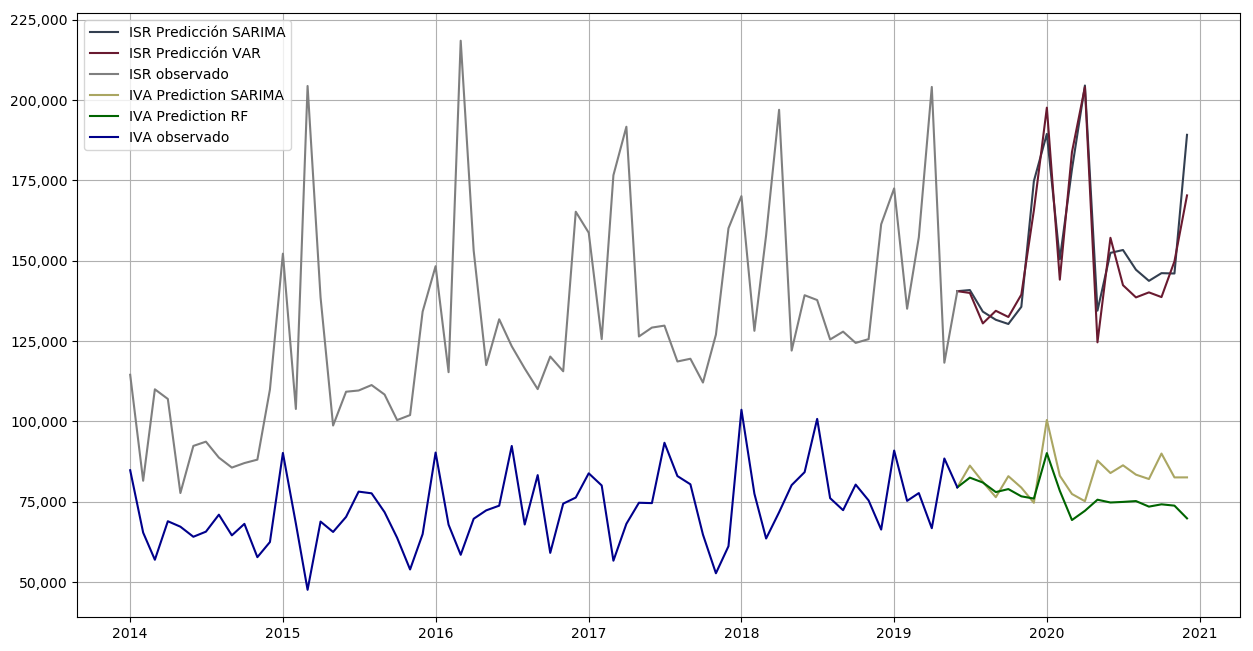
\includegraphics[scale = 0.5]{figures/pred_isr_iva}
\end{figure}

\begin{figure}[hbt!]
    \centering
     \caption{Impuesto a las importaciones e IEPS sin gasolina}
     \label{fig:pred_imp_ieps}
     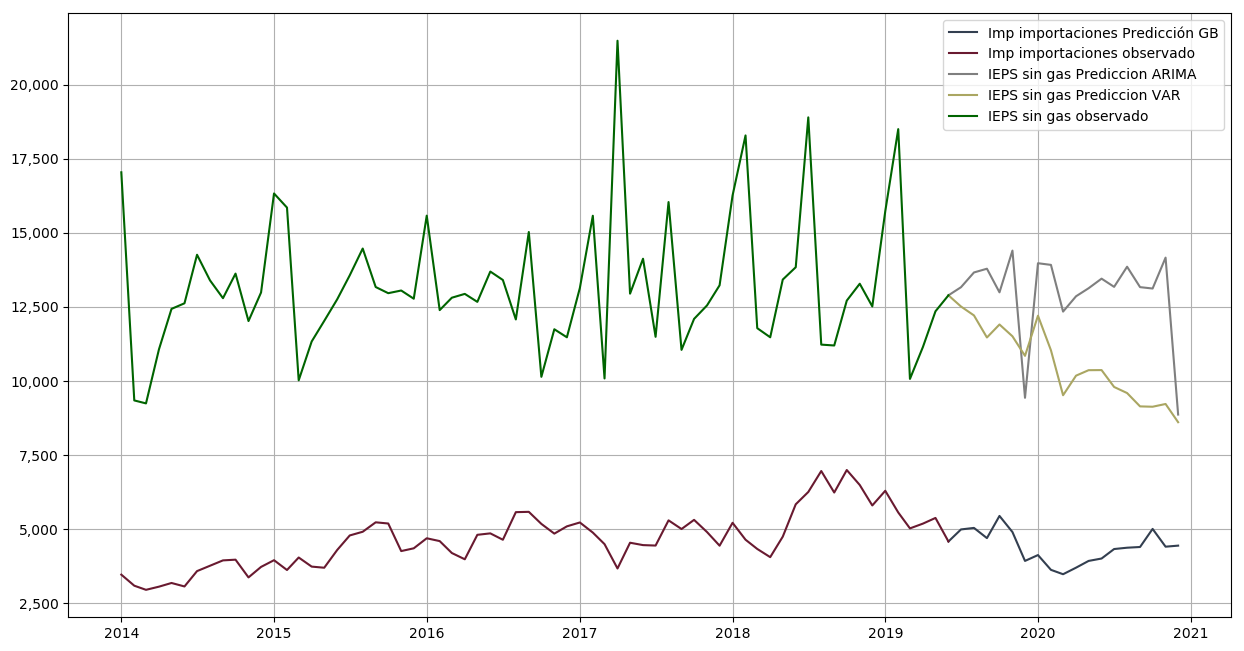
\includegraphics[scale = 0.5]{figures/pred_imp_ieps}
\end{figure}

Al convertir estas predicciones mensuales a anuales, obtenemos lo que se observa en la siguiente tabla: Estimamos un cierre de los ingresos tributarios ligeramente superior al estimado en la Ley de Ingresos que es de 3.311 billones de pesos. Estimamos implícitamente 306 MMDP de IEPS a las gasolinas, que es superior a los 269 MMDP estimados en la LIF, pero en línea con el comportamiento observado de alza en esos ingresos. De ISR estimamos entre 1,774 y 1781 billones de pesos, que es superior al programa entre 22 y 29 MMDP. De IVA, estimamos entre 955 y 957  MMDP que es alrededor de 40 MMDP por debajo de programa, compensando así el buen pronóstico del ISR. Finalmente, estimamos impuesto a las importaciones en 61 MMDP, y IEPS sin gasolina en un rango de 150 a 159 MMDP, 10 mil por debajo del programa en ambos casos. 
% Table generated by Excel2LaTeX from sheet 'Sheet1'
\begin{table}
\begin{tabular}{p{3em}p{3em}p{3em}p{3em}p{3em}}
\multicolumn{1}{p{6.415em}}{\textbf{Año}} & \multicolumn{1}{p{6.415em}}{\textbf{Ing trib (SARIMA)}} & \multicolumn{1}{p{6.415em}}{\textbf{Ing trib sin gas (SARIMA)}} & \multicolumn{1}{p{6.415em}}{\textbf{ISR (SARIMA)}} & \multicolumn{1}{p{6.415em}}{\textbf{ISR (VAR)}} \\ \hline \hline
2018 & 3,157,852.74  & 2,964,761.58  & 1,716,680.20  & 1,716,680.20  \\ \hline
2019 & 3,312,588.12  & 3,006,346.59  &  1,780,505.90  & 1,774,419.65   \\ \hline
2020 & 3,540,834.88  & 3,081,215.12  &  1,931,424.32  &  1,895,684.38  \\ \hline \hline
\end{tabular}%
\end{table}
\begin{table}[h]
\begin{tabular}{p{3em}p{3em}p{3em}p{3em}p{3em}p{3em}}
\multicolumn{1}{p{6.415em}}{\textbf{Año}}& \multicolumn{1}{p{6.415em}}{\textbf{IVA (SARIMA)}} & \multicolumn{1}{p{6.415em}}{\textbf{IVA (GB)}} & \multicolumn{1}{p{6.415em}}{\textbf{Imp. Importaciones (GB)}} & \multicolumn{1}{p{6.415em}}{\textbf{IEPS sin gas (ARIMA)}} & \multicolumn{1}{p{6.415em}}{\textbf{IEPS sin gas (VAR)}} \\ \hline \hline
2018 & 951,394.72  &           951,394.72  &              67,465.72  &           164,831.43  &           164,831.43  \\ \hline
2019 & 956,531.91  &           955,579.67  &              61,358.29  &           159,020.81  &           150,257.99  \\ \hline
2020 & 1,011,065.21  &           930,561.77  &              55,709.09  &           155,069.50  &           117,587.04  \\ \hline \hline
\end{tabular}%
\end{table}
\section*{Conclusiones}
El ejercicio permitió hacer un análisis de los ingresos tributarios y construir una herramienta predictiva que se basa en evidencia sólida del desempeño de los modelos. Vemos que los modelos econométricos tuvieron mejor desempeño que los modelos de \textit{Machine Learning}. Esto puede implicar de que la estructura impuesta por los modelos econométricos describe mejor a los ingresos tributarios que las estructuras que buscan crear los modelos que se estimaron. No obstante, es necesario recalcar que se excluyeron modelos del análisis, incluyendo a todos los que se denominan de \textit{Deep learning}. Son modelos muy valiosos que sería importante explorar en un futuro. 

Además, tal como se indicó al inicio, de este ejercicio se derivaron cuatro conclusiones. 
\begin{enumerate}
	\item La primera de ellas, es que la elasticidad de recaudación con respecto al Producto Interno Bruto es mayor a la unidad. Como se vio, es incluso superior a 2 para los ingresos que excluyen IEPS.
	\item La recaudación tributaria en valores netos es un proceso que se ve afectado fuertemente por acciones políticas que dificultan su predicción. De acuerdo expertos en la Secretaría de Hacienda, el flujo devoluciones y compensaciones del Servicio de Administración Tributaria (SAT) responde en gran medida a juego entre dos fuerzas: por un lado, existen presiones políticas para lograr los ingresos estipulados en la Ley de Ingresos de la Federación. Por otro lado, existen presiones de los grandes contribuyentes para obtener devoluciones y compensaciones de forma expedita para financiar sus operaciones. Este juego hace que el comportamiento de los ingresos netos se aleje de la lógica que explicaría el ciclo económico.
	\item Aunado a lo anterior, los ingresos por los diferentes impuestos difieren en su predictibilidad. De acuerdo con los modelos estimados, la recaudación neta por el ISR es mucho más predecible que la recaudación por IVA, Impuesto a las Importaciones e IEPS. Presumiblemente, esto es resultado de la naturaleza de cada uno de estos impuestos, y de la relevancia que tienen los gastos fiscales en cada uno de ellos.
	\item Los avances logrados por la UPIT, transitando hacia un mayor uso de las herramientas de análisis de información, hacia la automatización de procesos de análisis, y hacia la consolidación de bases de datos ordenadas, consistentes y confiables son de suma importancia. Otro de los proyectos realizados durante este Verano logró un sitio web para la consulta de datos de recaudación que será fundamental para el trabajo de análisis de política tributaria. De igual manera, las herramientas de descarga, limpieza, análisis y predicción, y las capacidades de \textit{Python} que se desarrollaron en el equipo analista que resultaron de este proyecto tienen el potencial de incrementar la productividad del equipo de análisis. Para continuar avanzando en esta dirección, el equipo identificó dos áreas estratégicas de inversión:
	\begin{enumerate}
		\item Invertir en la integración de Bases de Datos del SAT con la UPIT. Transitar de un modelo de envío de reportes mensuales por correo electrónico a un modelo en el que el equipo analista pueda consultar la información que la Tesorería de la Federación y el SAT administran en tiempo real. Este proceso de democratización de la información incrementará la productividad del equipo de la UPIT pues disminuirá las barreras que existen en el acceso de la información. Hoy en el mejor de los casos depende del simple envío de un reporte por parte de un área del SAT, pero en el peor de los casos, de semanas de espera por parte de la Unidad y de horas de trabajo por parte del equipo del SAT que ocurren después de una solicitud de información de la UPIT.
		\item Continuar con la capacitación del equipo en lenguajes de programación como \textit{Python} o \textit{R}. En estos meses de proyecto, donde se dieron capacitaciones semanales de \textit{Python} al equipo, se lograron avances muy importantes. Un analista que no tenía conocimientos de programación realizó su primer análisis de política tributaria en este lenguaje. El equipo analista está formado por los mejores economistas que están egresando actualmente, por lo que seguir invirtiendo en su capacitación en estas herramientas dará resultados cada vez más relevantes y más rápidos en la productividad.
\end{enumerate}
\end{enumerate}
\begin{landscape}
\section*{Anexo}

% Table generated by Excel2LaTeX from sheet 'Sheet1'
%\begin{longtable}{p{4em}p{4em}p{7em}p{16.165em}p{3.665em}rrrrrr}
% Table generated by Excel2LaTeX from sheet 'mejores_gral'
\begin{longtable}{p{5em}p{3.5em}p{13.165em}p{2.835em}rrrrrrr}
\caption{Precisión de los mejores modelos para cada variable según RMSE del periodo completo}\\ 
\textbf{variable} & \textbf{model} & \textbf{params} & \textbf{endog vars} & \multicolumn{1}{p{2.665em}}{\textbf{exog vars}} & \multicolumn{1}{p{2.915em}}{\textbf{mape first6}} & \multicolumn{1}{p{2.915em}}{\textbf{mape first18}} & \multicolumn{1}{p{2.915em}}{\textbf{mape last12}} & \multicolumn{1}{p{3.915em}}{\textbf{rmse first6}} & \multicolumn{1}{p{3.915em}}{\textbf{rmse last12}} & \multicolumn{1}{p{3.915em}}{\textbf{rmse first18}} \\
\hline \hline
 Ing. trib & ARIMA & order : (3, 0, 3)  & -     & 3     & 0.07  & 0.08  & 0.09  & 19656.34 & 26550.18 & 24226.09 \\
\hline
 Ing. trib & SARIMA & enforce invertibility : False,  enforce stationarity : False,  order : (2, 0, 2),  seasonal order : (1, 0, 1, 12)  & -     & 3     & 0.05  & 0.08  & 0.10  & 13313.50 & 31154.23 & 26314.33 \\
\hline
 Ing. trib & VAR   & ic :  bic ,  maxlags : 12,  trend :  c   & f     & 4     & 0.07  & 0.08  & 0.09  & 18827.34 & 32599.70 & 28665.61 \\
\hline
 Ing. trib & GB    & learning rate : 0.1,  max depth : 5,  n estimators : 1000,  random state : 1234,  subsample : 0.5  & -     & 5     & 0.08  & 0.20  & 0.26  & 23523.69 & 71850.93 & 59279.52 \\
\hline
 Ing. trib sin gas. & ARIMA & order : (4, 0, 5)  & -     & 1     & 0.06  & 0.06  & 0.06  & 15326.36 & 16866.31 & 16386.63 \\
\hline
 Ing. trib sin gas. & SARIMA & enforce invertibility : False,  enforce stationarity : False,  order : (2, 0, 2),  seasonal order : (1, 0, 1, 12)  & -     & 3     & 0.05  & 0.06  & 0.06  & 14085.01 & 18451.37 & 16993.47 \\
\hline
 Ing. trib sin gas. & VAR   & ic :  aic ,  maxlags : 12,  trend :  c   & f     & 4     & 0.08  & 0.06  & 0.06  & 19922.69 & 17812.45 & 18703.65 \\
\hline
 Ing. trib sin gas. & RF    & criterion :  mae ,  max depth : 5,  max features :  sqrt ,  min samples split : 10,  n estimators : 100,  n jobs : -1,  random state : 1234  & -     & 5     & 0.07  & 0.07  & 0.07  & 19103.10 & 22091.67 & 21819.67 \\
\hline
 Ing. trib sin gas. & GB    & learning rate : 0.1,  max depth : 5,  n estimators : 100,  random state : 1234,  subsample : 1.0  & -     & 5     & 0.08  & 0.08  & 0.08  & 19327.48 & 23233.96 & 22040.09 \\
\hline
 Ing. trib sin gas. & DT    & criterion :  mae ,  max depth : 5,  max features :  log2 ,  min samples split : 5,  random state : 1234  & e     & 5     & 0.10  & 0.12  & 0.14  & 24862.23 & 38706.20 & 34270.02 \\
\hline
 ISR  & VAR   & ic :  aic ,  maxlags : 12,  trend :  c   & d     & 3     & 0.06  & 0.06  & 0.07  & 9201.59 & 13365.20 & 11958.91 \\
\hline
 ISR  & SARIMA & enforce invertibility : False,  enforce stationarity : False,  order : (3, 0, 3),  seasonal order : (1, 0, 1, 12)  & -     & 2     & 0.06  & 0.09  & 0.11  & 8136.13 & 19009.22 & 15954.45 \\
\hline
 ISR  & ARIMA & order : (4, 0, 2)  & -     & 1     & 0.09  & 0.09  & 0.09  & 12538.98 & 17813.42 & 16013.68 \\
\hline
 ISR  & RF    & criterion :  mse ,  max depth : 50,  max features :  log2 ,  min samples split : 2,  n estimators : 100,  n jobs : -1,  random state : 1234  & a     & 5     & 0.07  & 0.10  & 0.11  & 11513.00 & 24025.60 & 20383.99 \\
\hline
 ISR  & GB    & learning rate : 0.1,  max depth : 5,  n estimators : 100,  random state : 1234,  subsample : 1.0  & e     & 5     & 0.09  & 0.14  & 0.17  & 12527.43 & 27041.28 & 22716.58 \\
\hline
 ISR  & DT    & criterion :  mae ,  max depth : 5,  max features :  log2 ,  min samples split : 5,  random state : 1234  & e     & 5     & 0.12  & 0.13  & 0.14  & 18019.58 & 29244.75 & 25647.05 \\
\hline
 IVA  & SARIMA & enforce invertibility : False,  enforce stationarity : False,  order : (2, 0, 1),  seasonal order : (1, 0, 1, 12)  & -     & 3     & 0.13  & 0.11  & 0.09  & 10065.17 & 8413.28 & 9034.53 \\
\hline
 IVA  & VAR   & ic :  fpe ,  maxlags : 12,  trend :  c   & a     & 3     & 0.13  & 0.11  & 0.10  & 10352.80 & 8874.40 & 9461.40 \\
\hline
 IVA  & ARIMA & order : (4, 0, 4)  & -     & 1     & 0.13  & 0.12  & 0.11  & 10728.77 & 10246.51 & 10404.70 \\
\hline
 IVA  & RF    & criterion :  mae ,  max depth : 50,  max features :  sqrt ,  min samples split : 2,  n estimators : 1000,  n jobs : -1,  random state : 1234  & e     & 5     & 0.13  & 0.12  & 0.11  & 10910.50 & 10063.65 & 10448.99 \\
\hline
 IVA  & GB    & learning rate : 0.1,  max depth : 5,  n estimators : 50,  random state : 1234,  subsample : 1.0  & b     & 5     & 0.15  & 0.12  & 0.11  & 11640.15 & 10043.41 & 10667.79 \\
\hline
 IVA  & DT    & criterion :  friedman mse ,  max depth : 1,  max features : None,  min samples split : 10,  random state : 1234  & e     & 5     & 0.13  & 0.13  & 0.12  & 10797.97 & 12240.75 & 12007.96 \\
\hline
 IEPS sin gas. & ARIMA & order : (5, 0, 1)  & -     & 2     & 0.18  & 0.18  & 0.18  & 2526.30 & 2638.72 & 2608.73 \\
\hline
 IEPS sin gas. & SARIMA & enforce invertibility : False,  enforce stationarity : False,  order : (2, 0, 2),  seasonal order : (1, 0, 1, 12)  & -     & 1     & 0.17  & 0.19  & 0.20  & 2409.77 & 2887.69 & 2724.33 \\
\hline
 IEPS sin gas. & VAR   & ic :  aic ,  maxlags : 12,  trend :  c   & c     & 3     & 0.16  & 0.21  & 0.24  & 2300.35 & 3430.34 & 3077.77 \\
\hline
 IEPS sin gas. & DT    & criterion :  mae ,  max depth : 20,  max features :  log2 ,  min samples split : 5,  random state : 1234  & -     & 5     & 0.35  & 0.29  & 0.25  & 5221.35 & 4307.34 & 4820.51 \\
\hline
 IEPS sin gas. & RF    & criterion :  mse ,  max depth : 5,  max features :  log2 ,  min samples split : 2,  n estimators : 1,  n jobs : -1,  random state : 1234  & e     & 5     & 0.38  & 0.32  & 0.29  & 5393.72 & 4907.48 & 5171.67 \\
\hline
 IEPS sin gas. & GB    & learning rate : 0.5,  max depth : 5,  n estimators : 1,  random state : 1234,  subsample : 1.0  & e     & 5     & 0.40  & 0.38  & 0.36  & 5664.22 & 5669.68 & 5683.37 \\
\hline
Imp. import. & RF    & criterion :  mse ,  max depth : 5,  max features :  log2 ,  min samples split : 2,  n estimators : 100,  n jobs : -1,  random state : 1234  & -     & 5     & 0.07  & 0.10  & 0.11  & 453.37 & 674.80 & 618.11 \\
\hline
Imp. import. & GB    & learning rate : 0.1,  max depth : 10,  n estimators : 1,  random state : 1234,  subsample : 0.5  & b     & 5     & 0.08  & 0.10  & 0.11  & 554.73 & 642.67 & 618.37 \\
\hline
Imp. import. & SARIMA & enforce invertibility : False,  enforce stationarity : False,  order : (2, 0, 3),  seasonal order : (1, 0, 1, 12)  & -     & 1     & 0.08  & 0.10  & 0.10  & 510.03 & 651.29 & 652.53 \\
\hline
Imp. import. & DT    & criterion :  mae ,  max depth : 5,  max features :  log2 ,  min samples split : 10,  random state : 1234  & -     & 5     & 0.09  & 0.11  & 0.12  & 592.19 & 711.18 & 663.92 \\
\hline
Imp. import. & VAR   & ic :  bic ,  maxlags : 12,  trend :  c   & b     & 3     & 0.09  & 0.10  & 0.10  & 578.89 & 646.72 & 664.22 \\
\hline
Imp. import. & ARIMA & order : (4, 0, 5)  & -     & 1     & 0.10  & 0.10  & 0.11  & 599.36 & 694.88 & 708.42 \\
\hline\hline
\end{longtable}%

\noindent
1 -	  mes 1 ,  mes 3 ,  mes 4 ,  mes 12 ,  year 2009 ,  year 2015 ,  semana santa ,  IVA ,  ISRP ,  ISRE  \\\\
2 -	  igae ,  mes 1 ,  mes 3 ,  mes 4 ,  mes 12 ,  year 2009 ,  year 2015 ,  semana santa ,  IVA ,  ISRP ,  ISRE  \\\\
3 -	  igae ,  inpc ,  tasa cetes 91 mensual ,  tc mensual ,  commodity price index ,  importaciones r ,  indic mens consumo ,  mes 1 ,  mes 3 ,  mes 4 ,  mes 12 ,  year 2009 ,  year 2015 ,  semana santa ,  IVA ,  ISRP ,  ISRE  \\\\
4 -	  commodity price index ,  cons price index us ,  ind prod ind us ,  tbill 3meses mensual ,  trade weighted exchange rate ,  year 2009 ,  year 2015 ,  semana santa ,  IVA ,  ISRP ,  ISRE  \\\\
5 -	Todas las variables descritas para modelos \textit{Machine Learning} \\\\\\
a -	   ISR ,  IVA  \\\\
b -	   ISR ,  IVA ,  Imp. import.  \\\\
c -	   ISR ,  IVA ,  IEPS sin gas. ,  Imp. import.  \\\\
d -	   ISR ,  Imp. import.  \\\\
e -	   ISR ,  IVA ,   Ing. trib sin gas. ,  IEPS sin gas. ,  Imp. import.  \\\\
f -	  igae sa ,  tc mensual ,  tasa cetes 91 mensual ,  inpc ,   Ing. trib ,  importaciones r ,  indic mens consumo 

\end{landscape}


\newpage
\section*{References}
\begin{hangparas}{.25in}{1}
Sabau, Hernán.(2011). \textit{Análisis Econométrico Dinámico. Una exploración para series de tiempo con el método econométrico.}\\
Box, George and Jenkins, G. M (1976). \textit{Time Series Analysis: Forecasting and Control.} San Francisco: Holden\\

Provost, Foster, and Tom Fawcett. (2013)\textit{Data Science for Business: What you need to know about data mining and data-analytic thinking.} " O'Reilly Media, Inc.",\\
\end{hangparas}

\end{document}
